\chapter{Recovery via convex programs}\label{ch:recovery_convex}

We left Chapter \ref{ch:graphs_signals_sampling} with an \emph{ill-posed} problem: retrieve $\mathbf{x}$ by observing $\mathbf{y} := \mathbf{Ax}$. Due to unsampled vertices, the measurement matrix $\mathbf{A}$ is rank-deficient, so it cannot be inverted. In other words, there is no way to distinguish, a priori, a signal $\mathbf{x}$ from all the points in the set $\left \{ \mathbf{z} \in \mathbb{R}^{n} : \mathbf{Az} = \mathbf{Ax} \right \}$.

The culprit for ill-posedness is the size of $\mathbb{R}^{n}$, the default search space. Linear algebra tells us that $\left \{ \mathbf{z} \in \mathbb{R}^{n} : \mathbf{Az} = \mathbf{Ax} \right \}$ has infinitely many points whenever $\mathbf{A}$ is non-invertible. But in this thesis we only care about \emph{piecewise-constant} signals, so we should not have to look for answers in the whole of $\mathbb{R}^{n}$. We should aim to find a smaller set $\mathcal{Z} \subset \mathbb{R}^{n}$ --- containing piecewise-constant signals --- for which the search space $\left \{ \mathbf{z} \in \mathcal{Z} : \mathbf{Az} = \mathbf{Ax} \right \}$ reduces to the singleton $\{ \mathbf{x} \}$. That is, restricted to $\mathcal{Z}$, the only vector with samples $\mathbf{y} = \mathbf{Ax}$ is $\mathbf{x}$ itself. There would be no loss of information by representing $\mathbf{x}$ in the compressed form $\mathbf{y}$.

In modern signal processing, the variational principle is a popular way to constrain the search space for inverse problems. First, one picks a function $f : \mathbb{R}^{n} \to \mathbb{R}$ that quantifies a key property of the signal $\mathbf{x}$ to be recovered. The function here is seen as a ``complexity cost'', taking small values for signals that look like $\mathbf{x}$ and large values otherwise. Then, one simply looks among the vectors agreeing with the measurements for the one that \emph{minimizes} $f$.
\begin{equation}
    \underset{\mathbf{z} \in \mathbb{R}^{n}}{\min} f(\mathbf{z}) \text{ subject to } \mathbf{Az = Ax}. \tag{P$f$} \label{eq:f_interpolation}
\end{equation}
We will call optimization programs like \eqref{eq:f_interpolation} \emph{interpolation} problems, because the ``penalty'' $f$ informs how to fill in the missing data, without changing the values of the sampled points.

Interpolation is fine if the measurements are noiseless. Noise demands that we adapt \eqref{eq:f_interpolation}, but a simple tweak is usually enough. Let $\mathbf{y} = \mathbf{Ax} + \mathbf{e}$ be the noisy samples and assume that we have (for some $q \geq 1$ and $\eta \geq 0$) the upper bound $\| \mathbf{e} \|_q^q \leq \eta$ on the noise component. Replace the equality constraint in \eqref{eq:f_interpolation} by $\| \mathbf{Az - y} \|_q^q \leq \eta$, allowing the recovered values at the sampled points to differ from the measurements, but restricting the difference to the noise level. The resulting \emph{regression} program~\footnote{I name it regression in contrast with the interpolation version, because the penalty $f$ potentially denoises the sampled values, in addition to filling in the missing data.} reads
\begin{equation}
    \underset{z \in \mathbb{R}^{n}}{\min} f(\mathbf{z}) \text{ subject to } \| \mathbf{Az - y} \|_q^q \leq \eta. \tag{P$f$-$\eta$} \label{eq:f_regression}
\end{equation}

Problem \eqref{eq:f_regression} actually generalizes \eqref{eq:f_interpolation}: it suffices to take $\eta = 0$ to get the latter from the former. Why then bother to define the two versions? This mostly has to do with Chapter \ref{ch:inexact_dual}, whose arguments apply an interpolation problem only. As that chapter contains the main theoretical contributions in this thesis, the numerical experiments in Chapter \ref{ch:numerical_tour} also consider only noiseless settings. But in Chapter \ref{ch:lower_bound_min_gain} we can work directly with regression, which allows more general conclusions. In any case, the text will make clear whether a statement is valid for a problem like \eqref{eq:f_regression} or solely for \eqref{eq:f_interpolation}.

Noise considerations aside, we still have to pick a function $f$ adapted to the graph signals that we care for. I proposed in Chapter \ref{ch:graphs_signals_sampling} that a piecewise-constant graph signal $\mathbf{x}$ is characterized by few jumps in value across the edges. Equivalently, the jump-set $\mathcal{S} := \operatorname{supp}\left ( \mathbf{Dx} \right )$ has small cardinality, or is sparse, using the language of \acrfull{cs}~\footnote{Some \acrshort{cs} researchers would also say that $\mathbf{x}$ is \emph{co-sparse} under the action of $\mathbf{D}$~\cite{nam2013}.}. We can write the cardinality of $\mathcal{S}$ as $|\mathcal{S}| = \|\mathbf{Dx}\|_0$, so the most direct proposal for a cost function appropriate to piecewise-constant graph signals would be the map $\mathbf{z} \overset{f}{\mapsto} \|\mathbf{Dz}\|_0$.

However, the $\ell_0$ ``norm'' is not convex, and it pays off to have a convex function in recovery programs. The reasons are both analytical and numerical. First, a convex $f$ turns \eqref{eq:f_regression} and \eqref{eq:f_interpolation} into convex problems, where every local minimum is a global minimum. Convexity brings with it a range of theoretical tools to analyze the properties of the solutions to the optimization problems. Second, convex problems have numerical solvers with \emph{convergence} guarantees. These solvers can approximate the global minimum with often relatively few iterations. Furthermore, the lack of sub-optimal local minima in convex problems ultimately decouples the numerical and analytical aspects of their solutions. In contrast, in non-convex problems such as the training of deep linear neural networks, the \emph{trajectories} of the gradient descent solver inform the properties of the solutions found in practice~\cite{arora2018a}. With decoupled analytical and numerical aspects, we can study convex programs independently of their practical implementation.

In \acrlong{cs}, the $\ell_1$-norm is the standard ``convexification'' of the $\ell_0$ ``norm''. This choice brings us to the \acrfull{gtv} interpolation decoder
\begin{equation}
    \underset{\mathbf{z} \in \mathbb{R}^{n}}{\min} \| \mathbf{D z} \|_1 \text{ such that } \mathbf{Ax = Az} \tag{P1} \label{eq:l1_interpolation}.
\end{equation}
Naturally, \eqref{eq:l1_interpolation} also has its noisy alternative,
\begin{equation}
    \underset{\mathbf{z} \in \mathbb{R}^{n}}{\min}  \| \mathbf{D z} \|_1 \text{ subject to } \| \mathbf{Az - y} \|_q^q \leq \eta \tag{P1-$\eta$} \label{eq:l1_regression}.
\end{equation}
which I call the \acrshort{gtv} regression problem. Most of this thesis is dedicated to dwelling on these two especial decoders.

But before that, the next section discusses some base conditions for unique and exact solution in the \emph{general} interpolation program \eqref{eq:f_interpolation}. In the process, I introduce the descent cone and the subdifferential of $\|\mathbf{D} \cdot\|_1$, sets that play a fundamental role towards linking the number of vertex samples with the success of \acrshort{gtv} minimization.

Following this, I argue why the \acrshort{gtv} semi-norm is a good convex surrogate to $\|\mathbf{D} \cdot\|_0$ as a signature for piecewise-constant graph signals. The reasoning is geometric, relying on the atomic status of $\|\mathbf{D} \cdot\|_1$. I also include a comparison with the Dirichlet form $\|\mathbf{D} \cdot\|_2^2$, using representer theorems to show that \acrshort{gtv} minimization is less dependent on the \emph{form} of the measurement matrix $\mathbf{A}$.

This chapter ends by connecting our recovery programs with the wider \acrlong{cs} literature. Indeed, we can see in \acrshort{gtv} minimization an instance of general co-sparse (or analysis-sparse) programs. What is exceptional in our setting is the sampling procedure. In \acrshort{cs}, Gaussian-like measurement vectors are the norm; comparatively little can be found on coordinate-sampled, co-sparse models. Much of the difficulty in the subsequent chapters \ref{ch:lower_bound_min_gain} and \ref{ch:inexact_dual} stems from the lack of tools to deal with our measurement matrix.


\section{When is the solution of convex interpolation unique?}

Due to the minimization principle, the only obstacles to $\mathbf{x}$ being the sole solution of \eqref{eq:f_interpolation} are the vectors $\mathbf{z} \in \mathbb{R}^{n}$ for which $f(\mathbf{z}) \leq f(\mathbf{x})$. To investigate the impact of these vectors, we can fix ourselves on $\mathbf{x}$ and check how much of $\mathbb{R}^{n}$ we cover by only moving in the directions that decrease $f$. The conic hull of these descent directions is called the descent cone.

\begin{definition}[Descent cone]
    Let $\mathbf{x}$ be a fixed point in $\mathbb{R}^{n}$. The descent cone of a convex function $f: \mathbb{R}^{n} \to \mathbb{R}$ at $\mathbf{x}$ is the set
    \begin{align}
        \mathcal{D}(f, \mathbf{x}) & := \operatorname{cone} \left ( \left\{ \mathbf{u} \in \mathbb{R}^{n} : f(\mathbf{x} + \mathbf{u}) \leq f(\mathbf{x}) \right\} \right ) \\
        & =: \bigcup_{\tau \geq 0} \left\{ \tau \mathbf{u} \in \mathbb{R}^{n} : f(\mathbf{x} + \mathbf{u}) \leq f(\mathbf{x}) \right\} .
    \end{align}
\end{definition}

Unique recovery in \eqref{eq:f_interpolation} then turns out to be a question about how the descent cone $\mathcal{D}(f, \mathbf{x})$ intersects the null space of the measurement matrix $\mathbf{A}$. The precise statement is given in Theorem \ref{thm:trivial_intersection_suffices}.

\begin{theorem}[\protect{\cite[Prop. 2.1]{chandrasekaran2012},\cite[Thm. 3]{kabanava2014}}]\label{thm:trivial_intersection_suffices}
    Vector $\mathbf{x}$ is the unique solution of problem \eqref{eq:f_interpolation} \emph{if and only if} the trivial intersection~\footnote{Both $\mathcal{D}(f, \mathbf{x})$ and $\operatorname{null} \left ( \mathbf{A} \right )$ contain at least $\mathbf{0}$, so ``trivial intersection'' highlights the situation when these sets agree only at the origin.} $\mathcal{D}(f, \mathbf{x}) \cap \operatorname{null} \left ( \mathbf{A} \right ) = \{ \mathbf{0} \}$ takes place.
\end{theorem}

The proof is standard but short, so I include it here.

\begin{proof}
    \pf
    \step{}{
        ``$\impliedby$'': Assume that $\mathcal{D}(f, \mathbf{x}) \cap \operatorname{null} \left ( \mathbf{A} \right ) = \{ \mathbf{0} \}$, and let $\mathbf{u} \in \mathbb{R}^{n}$ be such that $f(\mathbf{x} + \mathbf{u}) \leq f(\mathbf{x})$. Vector $\mathbf{x} + \mathbf{u}$ is thus a solution of problem \eqref{eq:f_interpolation} if $\mathbf{A}(\mathbf{x} + \mathbf{u}) = \mathbf{A}\mathbf{x}$. It follows that $\mathbf{x} + \mathbf{u} = \mathbf{x}$.
    }
        \begin{proof}
            \pf
            \step{}{$\mathbf{u} \in \mathcal{D}(f, \mathbf{x})$ by construction.}
            \step{}{$\mathbf{A}(\mathbf{x} + \mathbf{u}) = \mathbf{A}\mathbf{x} \implies \mathbf{u} \in \operatorname{null} \left ( \mathbf{A} \right )$}
            \step{}{$\mathbf{u} \in \mathcal{D}(f, \mathbf{x}) \cap \operatorname{null} \left ( \mathbf{A} \right ) \implies \mathbf{u} = 0$, by assumption.}~\qedsymbol
        \end{proof}

    \step{}{
        ``$\implies$'': Assume that $\mathbf{x}$ is the unique solution of \eqref{eq:f_interpolation}, and pick $\mathbf{u} \in \mathbb{R}^{n}$ such that $\mathbf{A}(\mathbf{x} + \mathbf{u}) = \mathbf{A}\mathbf{x}$. Then $\mathbf{u} \notin \mathcal{D}(f, \mathbf{x})$, unless $\mathbf{u} = \mathbf{0}$.
    }
        \begin{proof}
            \pf
            \step{}{$\mathbf{u} \in \operatorname{null} \left ( \mathbf{A} \right )$ by construction.}
            \step{}{If $\mathbf{u} \neq \mathbf{0}$, then $f(\mathbf{x} + \mathbf{u}) > f(\mathbf{x})$ because $\mathbf{x}$ is the unique feasible minimizer.}
            \step{}{$\mathbf{u} \in \mathcal{D}(f, \mathbf{x}) \iff \mathbf{u} \neq \mathbf{0}$}~\qedsymbol
        \end{proof}
    \qedstep{$\mathbf{x}$ is the unique solution of \eqref{eq:f_interpolation} $\iff$ $\mathcal{D}(f, \mathbf{x}) \cap \operatorname{null} \left ( \mathbf{A} \right ) = \{ \mathbf{0} \}$.}
\end{proof}

Theorem \ref{thm:trivial_intersection_suffices} is a geometric result, illustrated in Figure \ref{fig:illustration_trivial_intersection}. The cone $\mathcal{D}(f, \mathbf{x})$ is a deterministic object, the fruit of the signal we want to recover and its implicit modeling through function $f$. The null space of $\mathbf{A}$ is a random subspace: its exact orientation depends on which vertices are sampled in the graph.

\begin{figure}[H]
    \centering
    \begin{tikzpicture}[line cap=round, line join=round, scale=0.85, every node/.style={scale=0.85}]
    % frame
    \clip (5,5) circle (5);

    % origin
    \draw[fill=black] (5,5) circle (2pt);
    \draw[color=black] (5.2,5.2) node {$\mathbf{0}$};

    % null space
    \draw[line width=1pt, color=epfl-ardoise] (0,10) -- (10,0);
    \node at (6.5,3.5) [rotate=-45, anchor=south] {$\operatorname{null} \left ( \mathbf{A} \right )$};

    % noise cylinder
    \fill[color=epfl-canard, fill=epfl-canard, fill opacity=0.2]
    (0,9) -- (1,10) -- (10,1) -- (9,0) -- cycle;
    \draw[line width=1pt,dash pattern=on 2pt off 4pt,color=epfl-canard]
    (0,9) -- (9,0);
    \draw[line width=1pt,dash pattern=on 2pt off 4pt,color=epfl-canard]
    (1,10) -- (10,1);
    \node at (4.2,6.8) [color=epfl-canard, rotate=-45, anchor=south] {$\left \{ \mathbf{z} \in \mathbb{R}^{n} : \|\mathbf{Az} - \mathbf{y}\|_q^q \leq \eta \right\}$};

    % descent cone
    \fill[shift={(5,5)},line width=1pt,color=epfl-groseille,fill=epfl-groseille,fill opacity=0.2]
    (0,0) -- (-90:5cm) arc (-90:-180:5cm) -- (0,0);
    \draw[shift={(5,5)}, color=epfl-groseille] (-2.7,0.3) node {$\mathcal{D}( f, \mathbf{x})$};

    % sphere
    \draw (5,5) circle (4);
    \node at (6.5,0.75) {$\operatorname{bd}(\mathbb{B}_{q}^n)$};

\end{tikzpicture}
    \caption[The trivial intersection property]{Illustration of the trivial intersection property $\mathcal{D}(f, \mathbf{x}) \cap \operatorname{null} \left ( \mathbf{A} \right ) = \{ \mathbf{0} \}$.}
    \label{fig:illustration_trivial_intersection}
\end{figure}

Figure \ref{fig:illustration_trivial_intersection} points at an intuitive idea: the narrower the descent cone, the easier should be the for the trivial intersection to take place. The precise notion of width is discussed in Chapter \ref{ch:lower_bound_min_gain}, where we will also see that the same geometric idea can potentially be used to arrive at robust recovery guarantees for the \emph{regression} problem \eqref{eq:f_regression}. The reader may suspect that this is possible by examining how the blue slab $\left \{ \mathbf{z} \in \mathbb{R}^{n} : \|\mathbf{Az} - \mathbf{y}\|_q^q \leq \eta \right\}$ wraps around $\operatorname{null} \left ( \mathbf{A} \right )$. Potential regression solutions can distance themselves from $\mathbf{x}$ at most by approximately the noise level.

In the language of information theory, the trivial intersection property is the same as lossless dimension reduction using matrix $\mathbf{A}$. There is no ambiguity in representing $\mathbf{x}$ by $\mathbf{Ax}$, provided we use \eqref{eq:f_interpolation} as decoder. Gaussian matrices are known for their dimension reduction properties when applied to finite \cite{johnson1984} or sparse \cite{foucart2013} sets of vectors. And more recently broader classes of sub-Gaussian matrices have also been shown to behave as such~\cite{oymak2018}. Can one say the same about our coordinate sampling matrix $\mathbf{A}$? This is essentially the question studied in Chapter \ref{ch:lower_bound_min_gain}.

Specializing to \acrlong{gtv} interpolation, we can also obtain a simpler, \emph{necessary} condition for uniqueness. It involves the null space of $\mathbf{D}$ and is recorded in Proposition \ref{prop:trivial_null_necessary}.

\begin{proposition}\label{prop:trivial_null_necessary}
    If $\operatorname{null} \left ( \mathbf{D} \right ) \cap \operatorname{null} \left ( \mathbf{A} \right ) \neq \{ \mathbf{0} \}$, then problem \eqref{eq:l1_interpolation} has infinitely many solutions~\footnote{Actually, readers can examine the proof to convince themselves that the conclusion is valid whenever the interpolation problem \eqref{eq:f_interpolation} employs a function of the form $f(\cdot) = g(\mathbf{D} \cdot)$, where $g : \mathbb{R}^{N} \to \mathbb{R}$ is convex.}.
\end{proposition}

The subspace $\operatorname{null} \left ( \mathbf{D} \right )$ belongs to $\mathcal{D}(\|\mathbf{D} \cdot \|_1, \mathbf{x})$, so the trivial intersection property in Theorem \ref{thm:trivial_intersection_suffices} is strictly stronger. Nonetheless, Proposition \ref{prop:trivial_null_necessary} is a first glimpse on the compatibility required from the analysis and measurement operators if vector $\mathbf{x}$ is to be properly recovered.

\begin{proof}
    \pf\ Assume that $\mathbf{z}^\star$ is in the solution set of \eqref{eq:f_regression} and let $\mathbf{h}$ be an arbitrary point in the subspace $\operatorname{null} \left ( \mathbf{D} \right ) \cap \operatorname{null} \left ( \mathbf{A} \right ) \subset \mathbb{R}^{n}$. Note that $\mathbf{z}^\star + \mathbf{h}$ is feasible, as $\mathbf{A}(\mathbf{z}^\star + \mathbf{h}) - \mathbf{Ax} = \mathbf{A}\mathbf{z}^\star - \mathbf{Ax} = \mathbf{0}$. Furthermore, $\|\mathbf{D(z^\star + h)}\|_1 = \|\mathbf{Dz^\star}\|_1$, so $\mathbf{z}^\star + \mathbf{h}$ is also a solution. Since $\mathbf{h}$ was arbitrary and the subspace to which it belongs is not zero-dimensional, the claim holds.\hfill\qedsymbol
\end{proof}

Working with the descent cone is not the only way to derive uniqueness results for \eqref{eq:f_interpolation}. Readers familiar with optimization problems in Calculus know that maxima and minima of a differentiable function can be found where the gradient vanishes. The analogous object in the variational analysis of non-differentiable functions is the subdifferential set.

\begin{definition}[Subdifferential]
    Let $\mathbf{x}$ be a point in $\mathbb{R}^{n}$. The subdifferential of a convex function $f: \mathbb{R}^{n} \to \mathbb{R}$ at $\mathbf{x}$ is the set
    \begin{align}
        \partial f(\mathbf{x}) & := \left \{ \mathbf{u} \in \mathbb{R}^{n} : f(\mathbf{z}) - f(\mathbf{x}) \geq \langle \mathbf{u}, \mathbf{z} - \mathbf{x}\rangle, \enspace \forall \mathbf{z} \in \mathbb{R}^{n}\right \}.
    \end{align}
\end{definition}

The subdifferential $\partial f(\mathbf{x})$ is \emph{polar} to the closure of $\mathcal{D}(f, \mathbf{x})$ \cite[Thm. 23.7]{rockafellar1970}, meaning that $\langle \mathbf{v}, \mathbf{u} \rangle \leq 0$ whenever $\mathbf{u} \in \mean{\mathcal{D}(f, \mathbf{x})}$ and $\mathbf{v} \in \partial f(\mathbf{x})\}$. Intuitively, both sets share the origin, but ``point'' towards opposite directions. The trivial intersection property can be equivalently expressed in terms of the subdifferential under the guise of \acrfull{kkt} conditions. I explore this optic in Chapter \ref{ch:inexact_dual}.

\begin{figure}[H]
    \centering
    \begin{tikzpicture}[line cap=round, line join=round, scale=0.85, every node/.style={scale=0.85}]
    % frame
    \clip (5,5) circle (5);

    % origin
    \draw[fill=black] (5,5) circle (2pt);
    \draw[color=black] (5.0,5.3) node {$\mathbf{0}$};

    % null space
    \draw[line width=1pt, color=epfl-ardoise] (0,10) -- (10,0);
    \node at (6.5,3.5) [rotate=-45, anchor=south] {$\operatorname{null} \left ( \mathbf{A} \right )$};

    % range
    \draw[line width=1pt, color=epfl-ardoise] (0,0) -- (10,10);
    \node at (6.5,6.5) [rotate=45, anchor=south] {$\operatorname{range} \left ( \mathbf{A}^\top \right )$};

    % descent cone
    \fill[shift={(5,5)},line width=1pt,color=epfl-groseille,fill=epfl-groseille,fill opacity=0.2]
    (0,0) -- (-90:5cm) arc (-90:-180:5cm) -- (0,0);
    \draw[shift={(5,5)}, color=epfl-groseille] (-2.7,0.3) node {$\mathcal{D}( f, \mathbf{x})$};

    % subdifferential
    \fill[shift={(5,5)},line width=1pt,color=epfl-canard,fill=epfl-canard,fill opacity=0.2]
    (0,0) -- (0:5cm) arc (0:90:5cm) -- (0,0);
    \draw[shift={(5,5)}, color=epfl-canard] (2.7,-0.3) node {$\operatorname{cone}\left(\partial f(\mathbf{x})\right)$};

    % sphere
    \draw (5,5) circle (4);
    \node at (6.5,0.75) {$\operatorname{bd}(\mathbb{B}_{q}^n)$};

\end{tikzpicture}
    \caption[Polarity between descent cone and subdifferential]{Illustration of the polarity between the descent cone and the subdifferential of a convex function $f$. Exact recovery happens either if $\mathcal{D}(f, \mathbf{x})$ and $\operatorname{null} \left ( \mathbf{A} \right )$ intersect trivially, or equivalently if $\partial f(\mathbf{x})$ and $\operatorname{range} \left( \mathbf{A} \right)$ intersect non-trivially.}
    \label{fig:illustration_descent_cone_subdifferential}
\end{figure}

The subdifferential of the \acrshort{gtv} semi-norm has simple defining expressions, which I write down in the next proposition. I omit its proof because it is standard in variational analysis, and not very informative to us. Just recall that $\mathbf{P}_{\mathcal{S}} = \sum_{i \in \mathcal{S}} \tilde{\mathbf{e}}_i \tilde{\mathbf{e}}_i^\top$, denoting the coordinate projection indexed by set $\mathcal{S}$.

\begin{proposition}\label{prop:character_subdifferential_l1}
    Let $\mathcal{S} := \operatorname{supp}\left ( \mathbf{Dx} \right )$ for some matrix $\mathbf{D} \in \mathbb{R}^{N \times n}$ and some vector $\mathbf{x} \in \mathbb{R}^{n}$. A point $\mathbf{z} \in \mathbb{R}^{n}$ belongs to the subdifferential $\mathbf{z} \in \partial \|\mathbf{D} \cdot \|_1 (\mathbf{x})$ if and only if $\mathbf{z} = \mathbf{D}^\top \mathbf{w}$ for some $\mathbf{w} \in \mathbb{R}^{N}$ satisfying simultaneously
    \begin{align}
        \mathbf{P}_{\mathcal{S}} \mathbf{w} = \operatorname{sign} \left ( \mathbf{Dx} \right ), & \enspace \text{and}\\
        \left \| \left ( \mathbf{I}_N - \mathbf{P}_\mathcal{S} \right ) \mathbf{w} \right \|_{\infty} \leq 1.
    \end{align}
\end{proposition}

The polar relationship between descent cone and the subdifferential allow us deduce a corresponding expression for (the closure of) $\mathcal{D}(\| \mathbf{D} \cdot \|_1, \mathbf{x})$. The result, given as Proposition \ref{prop:character_l1_analysis_descent_cone}, has an accompanying proof in Appendix \ref{sec:proof_character_l1_analysis_descent_cone}.

\clearpage

\begin{proposition}\label{prop:character_l1_analysis_descent_cone}
    Let $\mathcal{S} := \operatorname{supp}\left ( \mathbf{Dx} \right )$. The topological closure of $\mathcal{D}(\| \mathbf{D} \cdot \|_1, \mathbf{x})$ can be written as
    \begin{equation}
        \mean{\mathcal{D}(\| \mathbf{D} \cdot \|_1, \mathbf{x})} = \left\{ \mathbf{u} \in \mathbb{R}^{n} : \left\langle \operatorname{sign} \left ( \mathbf{Dx} \right ), \mathbf{Du} \right\rangle \leq -\left\|(\mathbf{I}_N - \mathbf{P}_{\mathcal{S}}) \mathbf{Du}\right\|_1 \right\}.
    \end{equation}
\end{proposition}

This expression allows us to connect the trivial intersection in Theorem \ref{thm:trivial_intersection_suffices} with the so-called \emph{null-space property} commonly required in \acrlong{cs}~\cite[Ch. 4]{foucart2013}:
\begin{equation}
    \|\mathbf{P}_{\mathcal{S}} \mathbf{Du}\|_1 < \|(\mathbf{I}_N - \mathbf{P}_{\mathcal{S}}) \mathbf{Du}\|_1, \enspace \text{for all} \enspace \mathbf{u} \in \operatorname{null} \left ( \mathbf{A} \right ) \setminus \{\mathbf{0}\}.
    \label{eq:nsp}
\end{equation}
Note that $\| \mathbf{P}_{\mathcal{S}} \mathbf{Du}\|_1 \geq \left\langle \mathbf{P}_{\mathcal{S}}\operatorname{sign} \left ( \mathbf{Dx} \right ), \mathbf{Du} \right\rangle = \left\langle \operatorname{sign} \left ( \mathbf{Dx} \right ), \mathbf{Du} \right\rangle$, hence \eqref{eq:nsp} implies the trivial intersection $\mathcal{D}(\| \mathbf{D} \cdot \|_1, \mathbf{x}) \cap \operatorname{null} \left ( \mathbf{A} \right ) = \{\mathbf{0}\}$, through Proposition \ref{prop:character_l1_analysis_descent_cone}.


\section{Why \texorpdfstring{\acrshort{gtv}}{G-TV} minimization for piecewise-constant graph signals?}

In science, it is often a good idea to apply Occam's razor: among competing hypothesis, pick the simplest one. In signal processing, sparse linear models are among the simplest. Let $\mathbf{t}_1, \mathbf{t}_2, \dots \in \mathcal{T}$ be a set of vectors in $\mathbb{R}^{n}$, and $c_1, c_2, \dots \in \mathbb{R}$ be constants. A linear model of a signal $\mathbf{x}$, using the \emph{atoms} in $\mathcal{T}$ takes the form
\begin{equation}\label{eq:linear_model}
    \mathbf{x} = \sum_{i} c_i \mathbf{t}_i.
\end{equation}
The multiplying constants quantify the importance of each atom in describing $\mathbf{x}$. If only a few of the constants is different than zero, we say that the model is sparse. Equivalently, $\mathbf{x}$ is explained by only a few of the atoms in $\mathcal{T}$.

On the one hand, if we want the output of \eqref{eq:f_interpolation} to have have a sparse linear expression as \eqref{eq:linear_model}, then the set $\mathbf{x} + \mathcal{D}(f, \mathbf{x})$ gathering the potential solutions should contain the atoms in $\mathcal{T}$. On the other hand, Theorem \ref{thm:trivial_intersection_suffices} indicates that the descent cone should not be too ``wide'', lest it intersect with the null space of $\mathbf{A}$. The convex hull of $\mathcal{T}$, denoted $\operatorname{conv}(\mathcal{T})$, is the narrowest convex set containing $\mathcal{T}$, at least from the perspective of the angles at the atoms. Thus, whenever $\mathbf{x}$ is explained by combining few of such atoms, making $\mathcal{D}(f, \mathbf{x})$ the conic hull of $-\mathbf{x} + \operatorname{conv}(\mathcal{T})$ yields a fairly narrow cone. See Figure \ref{fig:illustration_convex_hull} for an illustration of this fact.

\clearpage

\begin{figure}[H]
    \centering
    \begin{tikzpicture}

    % frame
    \clip (1,1) circle (4);

    % axes
    %\draw[help lines, color=gray!30, dashed] (-5,-5) grid (5,5);

    % atoms
    \begin{scope}[every node/.style={circle, fill, color=black, scale=0.2, anchor=north east}]
        \node (0) at (0,0) {$\mathbf{0}$};
        \node (t1) at (3,3) {$\mathbf{t}_1$};
        \node (t2) at (2,0) {$\mathbf{t}_2$};
        \node (t3) at (0,-1) {$\mathbf{t}_3$};
        \node (t4) at (-1,0) {$\mathbf{t}_4$};
        \node (t5) at (0,2) {$\mathbf{t}_5$};
    \end{scope}

    % labels
    \begin{scope}
        \node[anchor=south west] at (0) {$\mathbf{0}$};
        \node[anchor=south west] at (t1) {$\mathbf{t}_1$};
        \node[anchor=north west] at (t2) {$\mathbf{t}_2$};
        \node[anchor=north] at (t3) {$\mathbf{t}_3$};
        \node[anchor=east] at (t4) {$\mathbf{t}_4$};
        \node[anchor=south east] at (t5) {$\mathbf{t}_5$};
    \end{scope}

    % convex hull
    \begin{scope}[every edge/.style={ultra thick, draw}, color=epfl-groseille]
        \path[-] (t1) edge (t2);
        \path[-] (t2) edge (t3);
        \path[-] (t3) edge (t4);
        \path[-] (t4) edge (t5);
        \path[-] (t5) edge (t1);
    \end{scope}

    % descent cone from convex hull
    \fill[color=epfl-groseille,fill=epfl-groseille, fill opacity=0.2]
    (t1) to (0,-6) -- (-6,0) to (t1);

    % a wider set
    \begin{scope}[every edge/.style={ultra thick, draw}, color=epfl-canard]
        \path[-] (t1) edge [bend left=15] (t2);
        \path[-] (t2) edge [bend left=15] (t3);
        \path[-] (t3) edge [bend left=15] (t4);
        \path[-] (t4) edge [bend left=15] (t5);
        \path[-] (t5) edge [bend left=15] (t1);
    \end{scope}

    % descent cone from wider set
    \fill[color=epfl-canard,fill=epfl-canard, fill opacity=0.2]
    (t1) to (3,-7) -- (-7,3) to (t1);

\end{tikzpicture}
    \caption[An atomic set and related descent cones]{An atomic set, $\mathcal{T} = \{\mathbf{t}_1, \dots, \mathbf{t}_5\}$, whose convex hull is bounded by the thick red lines. The thick blue lines form the boundary of a larger convex set containing the atoms in $\mathcal{T}$. Suppose that $\mathbf{x} = \mathbf{t}_1$. If $f$ is the gauge of $\operatorname{conv} \left ( \mathcal{T} \right )$, then the descent cone of this function at $\mathbf{x}$ has the same shape as the red cone. If, however, $f$ is the gauge of the larger convex set, then its descent cone at $\mathbf{x}$ is as wide as the blue cone.}
    \label{fig:illustration_convex_hull}
\end{figure}

The function $f$ for which $\mathcal{D}(f, \mathbf{x}) = \operatorname{cone} \left ( -\mathbf{x} + \operatorname{conv}(\mathcal{T}) \right )$ is the \emph{gauge} of $\operatorname{conv}(\mathcal{T})$~\cite{chandrasekaran2012}. This gauge is the map $\mathbf{z} \overset{f}{\mapsto} \|\mathbf{z}\|_{\mathcal{T}} := \inf \{ t > 0 : \mathbf{z} \in t \operatorname{conv}(\mathcal{T})\}$, which becomes a Minkowski \emph{norm} whenever $\mathcal{T}$ is symmetric about the origin. For a familiar example, the $\ell_1$ norm in $\mathbb{R}^{n}$ is the gauge of the convex hull of standard basis vectors $\mathbf{e}_1, \dots, \mathbf{e}_n$.

But what would be appropriate atomic set $\mathcal{T}$ for modelling piecewise-constant signals on graphs? Well, we have already a linear model for those signals in Chapter \ref{ch:graphs_signals_sampling}, using indicator vectors. Denote by $\mathcal{V}_1, \mathcal{V}_2, \dots$ all possible vertex subsets on the graph, and let $\mathbb{1}_{\mathcal{V}_1}, \mathbb{1}_{\mathcal{V}_2}, \dots$ be the corresponding indicator vectors. A piecewise-constant graph signal with $P$ pieces is then of the form
\begin{equation}\label{eq:linear_model_piecewise_constant}
    \mathbf{x} = \sum_{i} c_i \mathbb{1}_{\mathcal{V}_i},
\end{equation}
where we can always choose only $P$ of the constants $c_1, c_2, \dots$ to be non-zero. The matching vertex subsets are disjoint and represent each of the constant pieces of the signal. Given \eqref{eq:linear_model_piecewise_constant} and the discussion of the previous paragraphs, it makes sense then pick indicator vectors of vertex subsets as our signal atoms. This modeling by a sparse linear combination of indicator vectors also appears in Jung~\cite{jung2018} --- for example --- under the name of ``clustering hypothesis''.

The \acrshort{gtv} semi-norm induces a fairly narrow descent cone if $\mathbf{x}$ is described by a sparse combination of vertex-subset indicators. Formally, Proposition \ref{prop:extreme_points_gtv_ball} shows that such indicators are the ``extreme points''~\footnote{``Extreme points'' is in quotation marks because \glsname{Bgtv} does not actually have proper extreme points, consequence of the non-trivial null space of $\mathbf{D}$. Indeed, suppose $\mathbf{t}$ were an extreme point of \glsname{Bgtv}, and use some constant $c \in \mathbb{R}$ to create new points $\mathbf{s} := \mathbf{t} + c\mathbf{1}$ and $\mathbf{u} := \mathbf{t} - c\mathbf{1}$. Then, $\|\mathbf{Ds}\|_1 = \|\mathbf{Du}\|_1 = \|\mathbf{Dt}\|_1$, because $\operatorname{null} \left ( \mathbf{D} \right) \supset \operatorname{span} \left ( \mathbf{1} \right )$. This implies $\mathbf{s,t} \in \glsname{Bgtv}$. But at the same time, $\mathbf{t} = \frac{1}{2} (\mathbf{s} + \mathbf{u})$, so $\mathbf{t}$ cannot be an extreme point of \glsname{Bgtv}. The proposition goes around this problem by defining extreme points up to the null space of $\mathbf{D}$.} of the $\| \mathbf{D} \cdot \|_1$-ball. As a result the tip of the cone $\mathcal{D}(\|\mathbf{D} \cdot \|1, \mathbf{x})$ resembles the neighborhood of of a hyper-edge on the polyhedron $\operatorname{conv}(\{\mathbb{1}_{\mathcal{V}_1}, \mathbb{1}_{\mathcal{V}_2}, \dots\})$. The fewer atoms it takes to describe $\mathbf{x}$, the narrower this tip potentially is. Refer to Appendix \ref{sec:proof_extreme_gtv} for a proof of the proposition --- and a precise definition of ``up-to-additive-constant extreme points''.

\begin{proposition}[Extreme points of $\mathbb{B}_{\mathcal{G}-\acrshort{tv}}$, adapted from \protect{\cite{szlam2010}}]\label{prop:extreme_points_gtv_ball}
    A vector $\mathbf{t}^\star \in \mathbb{R}^{n}$ is an (up-to-additive-constant) extreme point of $\{ \mathbf{x} \in \mathbb{R}^{n} : \| \mathbf{Dx} \|_1 \leq 1\}$ \emph{if and only if} the entries of $\mathbf{t}^\star$ take on exactly two distinct values, $v_1 \neq v_2 \in \mathbb{R}$. In particular, such extreme points can be written as $\mathbf{t}^\star = (v_2 - v_1) \cdot \mathbb{1}_{\mathcal{S}_{v_2}(\mathbf{t}^\star)} + v_1 \mathbf{1}$, where $\mathcal{S}_{v_2}(\mathbf{t}^\star) := \{ i \in \mathbb{R}^{n} : t_i = v_2\}$.
\end{proposition}


\subsection{\texorpdfstring{\acrlong{gtv}}{Graph Total Variation} versus the Dirichlet form}\label{sec:gtv_versus_dirichlet}

I have just presented the \acrshort{gtv} semi-norm can be interpreted as the atomic gauge induced by indicator vectors of vertex subsets. But from the pure perspective of counting signal jumps, there is not much difference a priori between $\| \mathbf{Dx}\|_1 = \sum_{i,j} \sqrt{W_{ij}} |x_i - x_j|$ and the Dirichlet form~\footnote{The name ``Dirichlet form'' is inspired by noting that $\frac{1}{2}\mathbf{D}^\top \mathbf{D}$ is usually called the \emph{Laplacian} matrix $\mathbf{L}$~\cite{shuman2013}. Hence, $\|\mathbf{Dx}\|_2^2 = \mathbf{x}^{\top} \mathbf{L} \mathbf{x}$ is a Laplacian quadratic form.} $\|\mathbf{Dx}\|_2^2 = \sum_{i,j} W_{ij} (x_i - x_j)^{2}$ as signatures for piecewise-constant signals. How different it is to solve
\begin{equation}\label{eq:l2_regression}
    \underset{\mathbf{z} \in \mathbb{R}^{n}}{\min} \| \mathbf{Dz} \|_2^2 \text{ subject to } \| \mathbf{Az - y} \|_q^q \leq \eta,
\end{equation}
rather than \eqref{eq:l1_regression}? After all, a decoder similar to \eqref{eq:l2_regression} has been used by Puy \etal \cite{puy2016} for recovering sub-sampled, bandlimited~\footnote{Let $\mathbf{L} = \mathbf{U} \bm{\Lambda} \mathbf{U}^\top$ be the singular value decomposition of the graph Laplacian matrix, with eigenvector columns ordered from smallest to largest \acrshort{wrt} their respective eigenvalues. A signal is said to be \emph{$k$-bandlimited} if it lies in the span of the first $k$ eigenvectors in $\mathbf{U}$.} graph signals.

The answer I present in this section adapts the representer theorems of Unser \etal \cite{unser2016,unser2016a} to compare the \emph{form} of the points in the solution set of both $\ell_1$ and $\ell_2$ settings. A second, numerical perspective on the difference between \eqref{eq:l2_regression} and \eqref{eq:l1_regression} can be found in Chapter \ref{ch:numerical_tour}.

To place ourselves within the same context as Unser \etal, let us generalize a bit the regression problems \eqref{eq:l2_regression} and \eqref{eq:l1_regression}. Denote by $\mathcal{C}$ a convex, compact set in $\mathbb{R}^{m}$ and consider the program
\begin{equation}
    \mathcal{M}_p = \underset{\mathbf{z} \in \mathbb{R}^{n}}{\min} \| \mathbf{D z} \|_p^p \text{ such that } \mathbf{Az} \in \mathcal{C}. \label{eq:lp_reg_compact_set}
\end{equation}
Both \eqref{eq:l1_regression} and \eqref{eq:l1_regression} are particular instances of \eqref{eq:lp_reg_compact_set}, achieved by setting $\mathcal{C} = \{\mathbf{v} \in \mathbb{R}^{m} : \| \mathbf{v - Ax} \|_q^q \leq \eta\}$. This set is indeed convex and compact by virtue of being a scaled, translated norm ball.

The first representer theorem concerns the $\ell_1$ version of the general program \eqref{eq:lp_reg_compact_set}. Its proof, presented in Appendix \ref{ap:representer_l1}, is based on \cite[Theorem 19]{unser2016}.

\begin{theorem}\label{thm:l1_representer}
    Consider problem \eqref{eq:lp_reg_compact_set} with $p=1$ and assume that:
    \begin{enumerate}
        \item $\operatorname{null} \left ( \mathbf{D} \right ) \cap \operatorname{null} \left ( \mathbf{A} \right ) = \{ \mathbf{0} \}$.
        \item \label{ass:compact_convex} The set $\mathcal{C} \subset \mathbb{R}^{m}$ is convex and compact.
        \item \label{ass:feasible} The pre-image $\mathbf{A}^{-1}(\mathcal{C}) := \{\mathbf{z} \in \mathbb{R}^{n}: \mathbf{Az} \in \mathcal{C}\}$ is non-empty.
    \end{enumerate}
    Then, the extreme points of the solution set $\mathcal{M}_1$ are of the form
    \begin{equation}
        \mathbf{z}^\star = \mathbf{D}^+ \mathbf{a}^\star + \mathbf{b}^\star,
    \end{equation}
    where $\mathbf{a}^\star \in \mathbb{R}^{N}$ has at most $m$ non-zero coefficients, and $\mathbf{b}^\star \in \operatorname{null} \left ( \mathbf{D} \right )$.
\end{theorem}

The graph gradient matrix $\mathbf{D}$, mapping signals to edge differences, embodies our prior information that piecewise-constant graph signals vary little across edges. The columns of the  Moore-Penrose pseudo-inverse, $\mathbf{D}^+$, transfers the edge-differences perspective back to the vertex domain. The extreme points of the solution set of \eqref{eq:lp_reg_compact_set} are effectively explained by a small selection of columns of the pseudo-inverse. Consequently, the signals that we hope to recover have to be, in a sense, ``compatible'' with the network structure because $\mathbf{D}^+$ depends solely on the graph. For an example of compatible signal, turn to Figure \ref{fig:snc_udc_indicator_and_closest_pinv_atom}, where we meet once again the Swiss National Council graph introduced in Chapter \ref{ch:intro}. The presence of an atom of $\mathbf{D}^+$ so well-aligned with the party split indicates that the graph connections are a good predictor of whether a council member belongs or not to UDC. In other words, the party is a fairly well-defined community in the network.

\clearpage

\begin{figure}[H]
    \centering
    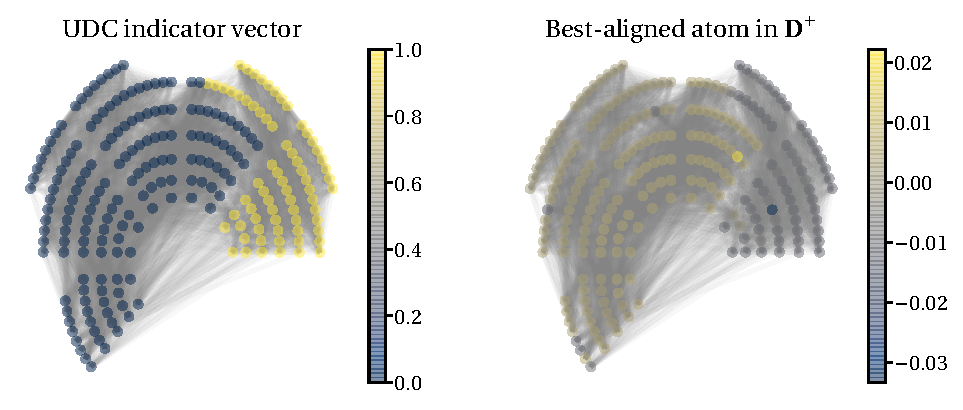
\includegraphics[width=0.9\textwidth]{snc_udc_indicator_and_closest_pinv_atom.pdf}
    \caption[A piecewise-constant signal that is compatible with the graph structure]{A piecewise-constant signal that is compatible with the graph structure. In the Swiss National Council graph depicted above, council members are linked by similarity in their voting patterns. The left image displays the indicator vector of the right-wing UDC party. Its best match among the columns (atoms) of the matrix $\mathbf{D}^+$, in terms of inner product, is shown on the right. Since $\mathbf{D}^+$ depends on the graph alone, the UDC party is fairly well encoded in the edge distribution and forms an effective community in the network.}
    \label{fig:snc_udc_indicator_and_closest_pinv_atom}
\end{figure}

Let us turn our attention now to the $\ell_2$ version of problem \eqref{eq:lp_reg_compact_set}. Unlike before, the measurement matrix $\mathbf{A}$ makes an appearance on the representer theorem.

\begin{theorem}\label{thm:l2_representer}
    Consider problem \eqref{eq:lp_reg_compact_set}, with $p=2$, and use the same set of assumptions as in Theorem \ref{thm:l1_representer}. Then, \emph{all} the points of the solution set $\mathcal{M}_2$ are of the form
    \begin{equation}
        \mathbf{z}^\star = \mathbf{D}^+ \mathbf{A}^\top \mathbf{v} + \mathbf{b}^\star,
    \end{equation}
    where $\mathbf{v} \in \mathbb{R}^{m}$ is a fixed vector, and $\mathbf{b}^\star \in \operatorname{null} \left ( \mathbf{D} \right )$.
\end{theorem}

Both theorems \ref{thm:l1_representer} and \ref{thm:l2_representer} include an unavoidable term in the null space of $\mathbf{D}$, but the solution set induced by the Dirichlet form depends explicitly on the measurement matrix $\mathbf{A}$. Unser \etal \cite{unser2016} use this contrast to argue that $\ell_1$ regularization is better at imposing prior information \emph{despite} the form of the measurements. This position will become even more appealing in Chapter \ref{ch:numerical_tour}, where I show that the recovery error of the Dirichlet form decoder is more sensitive to $\mathbf{A}$ than to the graph connections represented in $\mathbf{D}$.

\section{Relevant recovery results in the literature}

Problems with (potentially) redundant dictionaries~\footnote{The matrix $\mathbf{D}$ in $\|\mathbf{Dx}\|_1$ is often called dictionary or analysis operator because it maps $\mathbf{x}$ to a potentially sparse representation.} such as \eqref{eq:l1_regression} have been studied in \acrlong{cs} at least since Rauhut \etal \cite{rauhut2008} and Cand\`es \etal \cite{candes2011}. If $\mathbf{D}$ were a tight frame and $\mathbf{A}$ a Gaussian matrix, then the recovery error $\|\mathbf{z}^\star - \mathbf{x}\|_2$ of any solution $\mathbf{z}^\star$ to \eqref{eq:l1_regression} would be inversely proportional to $s := \|\mathbf{Dx}\|_0$, with an optimal dependence on the noise level \cite[Theorem 1.2]{candes2011}. The argument that Cand\`es \etal use to show this relies on $\mathbf{A}$ satisfying a certain $\mathbf{D}$-\acrlong{rip}. The number $(N - s)$~\footnote{Recall that $\mathbf{D} \in \mathbb{R}^{N \times n}$.} is sometimes called the cosparsity level of $\mathbf{x}$ under the analysis operator $\mathbf{D}$. Nam \etal \cite{nam2013} and Kabanava and Rauhut \cite{kabanava2015} are good places to find more results about cosparse models in compressed sensing. Still, these papers focus on frames for dictionaries Gaussian matrices measurements. Our graph gradient matrix is not a frame~\footnote{Due to its non-trivial null-space.}, and our measurement vectors are not Gaussian.

In Kabanava \etal~\cite{kabanava2015a} and Krahmer \etal~\cite{krahmer2017} we start to see difference operators being used as the analysis transform, but the measurements are still (sub-)Gaussian-like. Poon \cite{poon2015} also studies \acrlong{tv} minimization but in the context of weighted Fourier sampling. All of these works restrict themselves to signals lying on the Euclidean grid, so their difference matrix $\mathbf{D}$ can be interpreted as the graph gradient of the grid graph. I would like to be able to deal with more general graphs. Kabanava \etal \cite{kabanava2015a} attack the \acrlong{tv} problem by examining the descent cone of $\|\mathbf{D} \cdot\|_1$ and deriving a direct certificate of recovery, a strategy that we will explore in Chapter \ref{ch:lower_bound_min_gain}. Poon \cite{poon2015}, on the other hand, employs a golfing scheme, derived from the properties of the subgradient of $\|\mathbf{D} \cdot\|_1$, arriving at a so-called dual certificate. This is the line of work developed in Chapter \ref{ch:inexact_dual}, which is also greatly informed by the work of Boyer \etal \cite{boyer2019}.

One can also refer to Jung \etal \cite{jung2016, jung2017, jung2018} for a more network-oriented perspective on \acrlong{tv} recovery problems. Under their ``clustering hypothesis'', a piecewise-constant graph signal naturally induces a partition of the vertices into disjoint clusters. The sampled vertices are said to ``resolve'' the partition if they satisfy the \acrlong{nnsp} defined below.

\begin{definition}[\acrfull{nnsp}\protect{\cite{jung2016}}]
    The measurement matrix $\mathbf{A}$ satisfies the \acrshort{nnsp} \acrlong{wrt} an edge set $\mathcal{S} \subseteq \mathcal{E}$ if
    \begin{equation}
        \left \| \glsname{PS} \mathbf{D u} \right \|_1 \leq \frac{1}{2} \left \| (\mathbf{I}_n - \glsname{PS}) \mathbf{D u} \right \|_1,
    \end{equation}
    for any $\mathbf{u} \in \operatorname{null} \left ( \mathbf{A} \right ) \setminus \{ \mathbf{0} \}$.
\end{definition}

Similarly to other null-space properties in compressed sensing, the \acrshort{nnsp} is shown to imply exact recovery in the interpolation problem \eqref{eq:l1_interpolation}.

\begin{proposition}[\protect{\cite{jung2016}}]
    If $\mathbf{A}$ satisfies the \acrshort{nnsp} \acrshort{wrt} $\mathcal{S} = \operatorname{supp}\left ( \mathbf{D x} \right )$, then $\mathbf{x}$ is the unique solution \eqref{eq:l1_interpolation}.
\end{proposition}

Jung \textit{et al.} \cite{jung2016} give deterministic conditions upon which the sampled vertices resolve the partition induced by a piecewise signal of interest. These conditions look into the hop distances of sampled vertices to the borders of the partition, but do not otherwise inform how to design an optimal \emph{random} sampling for the recovery problem.

In this thesis, I approach optimal sampling design for the decoders \eqref{eq:l1_interpolation} and \eqref{eq:l1_regression} in a similar manner as Puy \etal \cite{puy2016} did. They showed that a type of coherence-weighted sampling can minimize the number of rows that $\mathbf{A}$ needs to represent an approximate isometry map for bandlimited graph signals. The decoder is naturally constructed by penalizing non-bandlimited vectors. In our case, we have decoders \eqref{eq:l1_interpolation} and \eqref{eq:l1_regression} that were hand-picked for another class of graph signals, piecewise-constant. But the optimal sampling design is still deduced by minimizing the sample complexity of the decoder with respect to the vertex sampling probabilities $\bm{\pi} = (\pi_i, \dots, \pi_n)$.

What kind of sample complexity expressions can one expect? Readers familiar with \acrlong{cs} might know that $m = \mathcal{O} \left( s \log (n/s) \right)$ random Gaussian measurements are enough to recover, with high probability, any $s$-sparse vector via $\ell_1$ minimization~\cite[Chapter 9]{foucart2013}. The ``sparsity-level'' in \acrfull{gtv} problems is $s := \|\mathbf{Dx}\|_0$, which is the number of edges in the jump-set $\mathcal{S} := \operatorname{supp}\left ( \mathbf{Dx} \right )$ of signal $\mathbf{x}$. Can one hope for sample complexity thresholds in \eqref{eq:l1_interpolation} that are proportional to $\|\mathbf{Dx}\|_0$? Surprisingly, such thresholds appear in the work of Lee \etal~\cite{lee2018}. They even apply for coordinate sampling, and have accompanying optimal designs. Why not just adapt Lee \etal's work to the context of graph signals to answer the main question in this thesis?

The reason is that Lee \etal~\cite{lee2018}'s bounds can be vacuous when dealing with graphs signals. I will show in Chapter \ref{ch:numerical_tour} examples where $|\mathcal{S}|$ is large in comparison to the number of vertices, but we can still successfully interpolate the respective signals using relatively few samples. For such large jump-sets, Lee \etal~\cite{lee2018} would prescribe a number of measurements, $m$, larger than the total number of vertices, $n$. Therefore our sample complexity should be more than just a function of the cardinality of the jump-set and potentially depend on the signal-to-be-recovered~\footnote{Results with this characteristic are often called ``non-uniform'' in \acrlong{cs}. They are named in contrast with results that are valid for a whole class of signals sharing a certain descriptive parameter. For example, any statement containing ``... for all $s$-sparse vectors ...'' is a uniform result.}.

This conclusion is not particularly new in the context of analysis-sparse (or co-sparse) models. Recent studies make a good case for considering only non-uniform guarantees whenever the decoder computes the $\ell_1$ norm in the image of a non-invertible analysis operator $\mathbf{D}$. For instance, Giryes \etal~\cite{giryes2015, giryes2015a} show that no algorithm can accurately recover a co-sparse signal from a number of measurements proportional to the signal's manifold dimension. Meanwhile, Genzel \etal~\cite{genzel2017a} construct two examples of analysis operators for which a signal has the same cosparsity level, but lead to completely different recovery thresholds~\footnote{Genzel \etal~\cite{genzel2017a} prescribe instead thresholds that depend on the partition of the Gram matrix $\mathbf{D} \mathbf{D}^\top$ by the support $\mathcal{S} := \operatorname{supp}\left ( \mathbf{Dx} \right )$. Through $\mathcal{S}$, their guarantee depends on $\mathbf{x}$, hence is non-uniform.}. Once again, those observations are to reinforce the fact that one should avoid naively using sample complexity thresholds proportional to $\|\mathbf{Dx}\|_0$ in problems like \eqref{eq:f_interpolation}.


\section{Summary and final notes}

The variational principle is a popular paradigm for recovering signals from subsampled linear measurements. Among all vectors satisfying the observation constraints, the returned solution is the one that minimizes a loss function $f$. This function is often chosen to be convex for analytical and numerical reasons.

There is also precedent in the literature for setting the search space directly, without resorting to a penalty $f$. Problems of the type ``$\underset{z \in \mathbb{R}^{n}}{\min} \| \mathbf{Az - y} \|_q^q \text{ subject to } \mathbf{z} \in \mathcal{K}$'', where $\mathcal{K}$ is a convex set, are sometimes called the $\mathcal{K}$-lasso \cite{plan2016}. Despite the difference at first sight, there is a $\rho > 0$ for which the $\mathcal{K}$-lasso becomes equivalent to \eqref{eq:f_regression} by setting $\mathcal{K} = \{\mathbf{z} \in \mathbb{R}^{n}: f(\mathbf{z}) \leq \rho \}$~\footnote{This can be proved by the method of Lagrange multipliers \cite[Chapter 5]{boyd2009}.}. Some researchers, like Bora \etal~\cite{bora2017a}, might even use non-convex constraint sets $\mathcal{K}$. They set out to recover images of human faces from few pixel measurements, having access to a pre-trained Generative Adversarial Network (GAN). This GAN excels in creating natural-looking faces, so Bora \etal argue that its range can be used as the recovery search space. It is an implicit way to avoid points in $\mathbb{R}^{n}$ that do not look like human faces, but it definitely makes the problem harder to study mathematically.

The \acrshort{gtv} semi-norm is a good penalty choice for recovering piecewise-constant signals on graphs. These signals have a sparse representation in terms of the extreme points of the \acrshort{gtv} ball. As a result, $\mathcal{D}(\| \mathbf{D} \cdot \|_1, \mathbf{x})$ should be fairly narrow when $\mathbf{x}$ is piecewise constant, making it easier for a trivial intersection with $\operatorname{null} \left ( \mathbf{A} \right )$ to take place. Ultimately, the trivial intersection is what guarantees the exact recovery of $\mathbf{x}$ from $\mathbf{Ax}$. I have also argued that minimizing $\|\mathbf{D} \cdot\|_1$ is preferable to minimizing $\|\mathbf{D} \cdot\|_2^2$ if we want solutions less dependent on the form of the measurement matrix.

Our main decoders, \eqref{eq:l1_interpolation} and \eqref{eq:l1_regression}, fall under the scope of co-sparse models in \acrlong{cs}. But the most relevant work in this field (Lee \etal~\cite{lee2018}) prescribes sample complexity bounds that are potentially vacuous when dealing with graph signals. In the end, I have to reach new recovery guarantees from scratch, with the next two chapters compiling attempts to do so. Chapter \ref{ch:lower_bound_min_gain} deals with a gain functional certifying that the descent cone $\mathcal{D}(\| \mathbf{D} \cdot \|_1, \mathbf{x})$ and the subspace $\operatorname{null} \left ( \mathbf{A} \right )$ intersect only at $\mathbf{0}$. In parallel, Chapter \ref{ch:inexact_dual} uses the characteristics of the subdifferential $\partial \| \mathbf{D} \cdot \|_1(\mathbf{x})$ as a blueprint to iteratively build a recovery certificate.

\clearpage

\begin{subappendices}
    \section{Geometry of the \texorpdfstring{\acrshort{gtv}}{G-TV} semi-norm}

    \subsection{Proof of Proposition \ref{prop:character_l1_analysis_descent_cone}}\label{sec:proof_character_l1_analysis_descent_cone}
    Here I adapt \cite[Lemma 4.1]{krahmer2019}, where Krahmer and St\"{o}ger characterize the descent cone of the matrix spectral norm. But first, let me precise the notion of polarity for cones.

\begin{definition}[Polar cone]\label{def:polar_cone}
    Let $\mathcal{K} \subset \mathbb{R}^{n}$ be a cone. The corresponding polar cone, denoted $\mathcal{K}^{\mathsf{o}}$, is the set
    \begin{equation}
        \mathcal{K}^{\mathsf{o}} := \{ \mathbf{v} \in \mathbb{R}^{n} : \langle \mathbf{v}, \mathbf{u} \rangle \leq 0, \forall \mathbf{u} \in \mathcal{K}\}.
    \end{equation}
\end{definition}

I will say that a vector $\mathbf{v}$ is polar to a set $\mathcal{S}$ if $\langle \mathbf{v}, \mathbf{s}\rangle \leq 0, \forall \mathbf{s} \in \mathcal{S}$. Similarly, $\mathbf{v}$ is polar to another vector $\mathbf{u}$ if $\langle \mathbf{v}, \mathbf{u}\rangle \leq 0$.

\begin{proof}
    \pf\ The desired expressions are a consequence of the subdifferential $\partial \|\mathbf{D} \cdot\|_1(\mathbf{x})$ being polar to $\mean{\mathcal{D}(\| \mathbf{D} \cdot \|_1, \mathbf{x})}$ \cite[Thm. 23.7]{rockafellar1970}. Recall from Proposition \ref{prop:character_subdifferential_l1} that $\mathbf{v} \in \partial \|\mathbf{D} \cdot\|_1(\mathbf{x})$ if and only if $\mathbf{v} = \mathbf{D}^\top \operatorname{sign} \left ( \mathbf{Dx} \right ) + \mathbf{D}^\top (\mathbf{I}_N - \mathbf{P}_{\mathcal{S}}) \mathbf{w}$, for some $\mathbf{w} \in \mathbb{R}^{N}$ satisfying $\left\|(\mathbf{I}_N - \mathbf{P}_{\mathcal{S}}) \mathbf{w}\right\|_\infty \leq 1$. We then split the argument in two parts:

    \step{}{
        ``$\impliedby$'': If $\left\langle \operatorname{sign} \left ( \mathbf{Dx} \right ), \mathbf{Du} \right\rangle \leq -\left\|(\mathbf{I}_N - \mathbf{P}_{\mathcal{S}}) \mathbf{Du}\right\|_1$ then $\mathbf{u} \in \mean{\mathcal{D}(\| \mathbf{D} \cdot \|_1, \mathbf{x})}$.
    }
        \begin{proof}
            \pf\ For any given $\mathbf{v} \in \mean{\mathcal{D}(\| \mathbf{D} \cdot \|_1, \mathbf{x})}\polar$, directly compute
            \begin{align*}
                \langle \mathbf{v}, \mathbf{u} \rangle & = \left\langle \mathbf{D}^\top \operatorname{sign} \left( \mathbf{Dx} \right) + \mathbf{D}^\top (\mathbf{I}_N - \mathbf{P}_{\mathcal{S}}) \mathbf{w}, \mathbf{u} \right\rangle \\
                & = \left\langle \operatorname{sign} \left ( \mathbf{Dx} \right ), \mathbf{Du} \right\rangle + \left\langle (\mathbf{I}_N - \mathbf{P}_{\mathcal{S}}) \mathbf{w}, \mathbf{Du} \right \rangle \\
                & \leq \left\langle \operatorname{sign} \left ( \mathbf{Dx} \right ), \mathbf{Du} \right\rangle + \left\|(\mathbf{I}_N - \mathbf{P}_{\mathcal{S}}) \mathbf{Du}\right\|_1 \cdot \underbrace{\left\|(\mathbf{I}_N - \mathbf{P}_{\mathcal{S}}) \mathbf{w}\right\|_\infty}_{\leq 1} & \comment{H\"older inequality} \\
                & \leq 0. & \comment{Assumption}
            \end{align*}
            Therefore, $\mathbf{u}$ is polar to $\mean{\mathcal{D}(\| \mathbf{D} \cdot \|_1, \mathbf{x})}\polar$, meaning $\mathbf{u} \in \mean{\mathcal{D}(\| \mathbf{D} \cdot \|_1, \mathbf{x})}$.\hfill\qedsymbol
        \end{proof}

    \step{}{
        ``$\implies$'': If $\mathbf{u} \in \mean{\mathcal{D}(\| \mathbf{D} \cdot \|_1, \mathbf{x})}$ then $\left\langle \operatorname{sign} \left ( \mathbf{Dx} \right ), \mathbf{Du} \right\rangle \leq -\left\|(\mathbf{I}_N - \mathbf{P}_{\mathcal{S}}) \mathbf{Du}\right\|_1$.
    }
        \begin{proof}
            \pf\
            \step{}{
                Pick a vector $\mathbf{w} \in \mathbb{B}_{\infty}^N$ for which $\langle \mathbf{w}, (\mathbf{I}_N - \mathbf{P}_{\mathcal{S}}) \mathbf{Du}\rangle = \left\|(\mathbf{I}_N - \mathbf{P}_{\mathcal{S}}) \mathbf{Du}\right\|_1$. Then $\mathbf{v} = \mathbf{D}^\top \operatorname{sign} \left ( \mathbf{Dx} \right ) + \mathbf{D}^\top (\mathbf{I}_N - \mathbf{P}_{\mathcal{S}}) \mathbf{w}$ is a valid subgradient in $\partial \|\mathbf{D} \cdot\|_1(\mathbf{x})$, because
                \begin{equation*}
                    \left\|(\mathbf{I}_N - \mathbf{P}_{\mathcal{S}}) \mathbf{w}\right\|_\infty \leq \underbrace{\left\|(\mathbf{I}_N - \mathbf{P}_{\mathcal{S}})\right\|_\infty}_{\leq 1} \cdot \underbrace{\left\|\mathbf{w}\right\|_\infty}_{\leq 1} \leq 1.
                \end{equation*}
            }
            \step{}{
                Since $\mathbf{v} \in \partial \|\mathbf{D} \cdot\|_1(\mathbf{x})$ is polar to $\mean{\mathcal{D}(\| \mathbf{D} \cdot \|_1, \mathbf{x})}$, we conclude that
                \begin{align*}
                    0 & \geq \langle \mathbf{u}, \mathbf{v} \rangle & \comment{Assumption} \\
                    & = \left\langle \mathbf{D}^\top \operatorname{sign} \left( \mathbf{Dx} \right) + \mathbf{D}^\top (\mathbf{I}_N - \mathbf{P}_{\mathcal{S}}) \mathbf{w}, \mathbf{u} \right\rangle \\
                    & = \left\langle \operatorname{sign} \left ( \mathbf{Dx} \right ), \mathbf{Du} \right\rangle + \left\|(\mathbf{I}_N - \mathbf{P}_{\mathcal{S}}) \mathbf{Du}\right\|_1. & \comment{Choice of $\mathbf{w}$}
                \end{align*}
            }
            \qedsymbol
        \end{proof}
    \qedstep
\end{proof}

    \subsection{Proof of Proposition \ref{prop:extreme_points_gtv_ball}}\label{sec:proof_extreme_gtv}
    I will need to establish some notation before delving into the argument.

\begin{definition}[Graph cut]
    The \emph{graph cut} associated with two vertex sets $\mathcal{S}_1, \mathcal{S}_2 \subset [n]$ is the set
    \begin{equation}
        \operatorname{cut}\left(\mathcal{S}_1, \mathcal{S}_2\right) := \left\{ e = \left(v_i, v_j\right) \in \mathcal{E} : (i \in \mathcal{S}_1 \wedge j \in \mathcal{S}_2) \vee (j \in \mathcal{S}_1 \wedge i \in \mathcal{S}_2)\right\}.
    \end{equation}
    We also define the size of $\operatorname{cut}\left(\mathcal{S}_1, \mathcal{S}_2\right)$ to be
    \begin{equation}
        \left|\operatorname{cut}\left(\mathcal{S}_1, \mathcal{S}_2\right)\right| := \sum_{i \in \mathcal{S}_1} \sum_{j \in \mathcal{S}_2} \sqrt{W_{ij}}.
    \end{equation}
\end{definition}

\begin{definition}[Up-to-additive-constant extreme point]
    We say that $\mathbf{t} \in \mathcal{S}$ is an up-to-additive-constant extreme point of $\mathcal{S}$ when we can write $\mathbf{t} = \beta \mathbf{s} + (1 - \beta) \mathbf{u}$, using $\beta \in (0,1)$ and $\mathbf{s}, \mathbf{u} \in \mathcal{S}$, only if $\mathbf{s} - \mathbf{t} = c_s \mathbf{1}$ and $\mathbf{u} - \mathbf{t} = c_u \mathbf{1}$, for some constants $c_s, c_u \in \mathbb{R}$.
\end{definition}

Lastly, define also the following \emph{level sets} of $\mathbf{t} \in \mathbb{R}^{n}$, indexed by $v \in \mathbb{R}$:
\begin{align}
    \mathcal{S}_{v}(\mathbf{t}) := \{i \in \mathbb{R}: t_i = v\} \\
    \mathcal{S}_{v^{+}}(\mathbf{t}) := \{i \in \mathbb{R}: t_i > v\} \\
    \mathcal{S}_{v^{-}}(\mathbf{t}) := \{i \in \mathbb{R}: t_i < v\}.
    \end{align}

I will prove a slightly stronger claim than the one stated in the main text: the up-to-additive-constants extreme points $\mathbf{t}^\star$ of \glsname{Bgtv} are of the form
\begin{equation}
    \mathbf{t}^\star = |\operatorname{cut}(\mathcal{S}_{v_1}(\mathbf{t}^\star), \mathcal{S}_{v_2}(\mathbf{t}^\star))| \cdot \mathbb{1}_{\mathcal{S}_{v_2}(\mathbf{t}^\star)} + v_1 \mathbf{1}.
\end{equation}
The argument is adapted from Szlam \etal~\cite{szlam2010}.

\begin{proof}
    \pf\  Let $v_1 < v_2 < \dots < v_d \in \mathbb{R}$ be all the distinct values taken by the coordinates of some $\mathbf{t} \in \mathbb{R}^{n}$. Trivially, $1 \leq d \leq n$. I will split the argument into the cases $d = 1$, $d = 2$, and $d \geq 3$, and show that $\mathbf{t}$ is an extreme point of \glsname{Bgtv} if and only if $d = 2$. The precise expression for $\mathbf{t}^\star$ will appear as a consequence of the computations in the proof.

    \step{}{If $d = 1$, $\mathbf{t}$ is not an extreme point of \glsname{Bgtv}.}
        \begin{proof}
            \pf\ Vector $\mathbf{t} = v_1 \mathbf{1}$ is constant, so $\|\mathbf{Dt}\|_1 = \sum_{(i,j)} \sqrt{W_{i,j}} |v_1 - v_1| = 0$. Since $\|\mathbf{Dt}\|_1 < 1$, vector $\mathbf{t}$ cannot be an extreme point of \glsname{Bgtv}.
        \end{proof}

    \step{}{If $d \geq 3$ and $\|\mathbf{Dt}\|_1 = 1$, $\mathbf{t}$ is still not an extreme point of \glsname{Bgtv}.}
        \begin{proof}
            \pf\ I will construct perturbations $\mathbf{s} := \mathbf{t} + \varepsilon_p \mathbb{1}_{\mathcal{S}_{v_p}(\mathbf{t})} - \varepsilon_q \mathbb{1}_{\mathcal{S}_{v_q}(\mathbf{t})}$ and $\mathbf{u} := \mathbf{t} - \varepsilon_p \mathbb{1}_{\mathcal{S}_{v_p}(\mathbf{t})} + \varepsilon_q \mathbb{1}_{\mathcal{S}_{v_q}(\mathbf{t})}$, for some small $\varepsilon_p, \varepsilon_q > 0$ and some $v_p, v_q \in \{v_1, \dots, v_d\}$. With these constructions, I show that $\mathbf{s}, \mathbf{u} \in \glsname{Bgtv}$. Since $\mathbf{t} = \frac{1}{2}\mathbf{s} + \frac{1}{2}\mathbf{u}$, this will imply that $\mathbf{t}$ cannot be an extreme point of \glsname{Bgtv}.
            \step{}{
                Note first that if we pick any positive $\varepsilon < \underset{k \neq l \in [d]}{\min} \enspace |v_k - v_l|$ the effect of the perturbation $\varepsilon \mathbb{1}_{\mathcal{S}_{v}(\mathbf{t})}$ decouples from $\| \mathbf{Dt} \|_1$:
                \begin{align*}
                    \| \mathbf{D} (\mathbf{t} + \varepsilon \mathbb{1}_{\mathcal{S}_{v}(\mathbf{t})}) \|_1 & = \sum_{(i,j) \in \mathcal{E}} \sqrt{W_{ij}} \left |t_i - t_j + \varepsilon \mathbb{1}_{\mathcal{S}_{v}(\mathbf{t})}(i) - \varepsilon \mathbb{1}_{\mathcal{S}_{v}(\mathbf{t})}(j) \right | \\
                    & = 2 \sum_{i \in \mathcal{S}_{v^{-}(\mathbf{t})}}\sum_{j \in \mathcal{S}_{v}(\mathbf{t})} \sqrt{W_{ij}} \underbrace{|t_i - t_j - \varepsilon|}_{= t_j - t_i + \varepsilon} \\
                    & \quad + 2 \sum_{i \in \mathcal{S}_{v}(\mathbf{t})}\sum_{j \in \mathcal{S}_{v}(\mathbf{t})} \sqrt{W_{ij}} |t_i - t_j| \\
                    & \quad + 2\sum_{i \in \mathcal{S}_{v}(\mathbf{t})}\sum_{j \in \mathcal{S}_{v^{+}}(\mathbf{t})} \sqrt{W_{ij}} \underbrace{|t_i - t_j + \varepsilon|}_{= t_j - t_i - \varepsilon} \\
                    & = \| \mathbf{Dt} \|_1 + \varepsilon \left ( \underbrace{\left [ \sum_{i \in \mathcal{S}_{v^{-}}(\mathbf{t})}\sum_{j \in \mathcal{S}_{v}(\mathbf{t})} \sqrt{W_{ij}} \right ]}_{=: \left|\operatorname{cut}\left(\mathcal{S}_{v^{-}}(\mathbf{t}), \mathcal{S}_{v}(\mathbf{t})\right)\right|} - \underbrace{\left [ \sum_{i \in \mathcal{S}_{v}(\mathbf{t})}\sum_{j \in \mathcal{S}_{v^{+}}(\mathbf{t})} \sqrt{W_{ij}} \right ]}_{=: \left|\operatorname{cut}\left(\mathcal{S}_{v^{+}}(\mathbf{t}), \mathcal{S}_{v}(\mathbf{t})\right)\right|} \right ). \\
                \end{align*}
            }
            \step{}{
                Therefore, if we pick $\varepsilon_p, \varepsilon_q < \frac{1}{2} \underset{k \neq l \in [d]}{\min} \enspace |v_k - v_l|$, we can write the \acrshort{gtv} semi-norm of $\mathbf{s}$ as
                \begin{align*}
                    \| \mathbf{Ds} \|_1 & = \left \| \mathbf{D} \left (\mathbf{t} + \varepsilon_p \mathbb{1}_{\mathcal{S}_{v_p}(\mathbf{t})} - \varepsilon_q \mathbb{1}_{\mathcal{S}_{v_q}(\mathbf{t})} \right ) \right \|_1 \\
                    & = \underbrace{\| \mathbf{Dt} \|_1}_{=1} + \varepsilon_p \left ( \left|\operatorname{cut}(\mathcal{S}_{v_p^{-}(\mathbf{t})}, \mathcal{S}_{v_p}(\mathbf{t})) \right| - \left|\operatorname{cut}(\mathcal{S}_{v_p^{+}(\mathbf{t})}, \mathcal{S}_{v_p}(\mathbf{t}))\right| \right ) \\
                    & \qquad\qquad\ - \varepsilon_q \left ( \left|\operatorname{cut}(\mathcal{S}_{v_q^{-}(\mathbf{t})}, \mathcal{S}_{v_q}(\mathbf{t}))\right| - \left|\operatorname{cut}(\mathcal{S}_{v_q^{+}(\mathbf{t})}, \mathcal{S}_{v_q}(\mathbf{t}))\right| \right ) \\
                \end{align*}
                and, similarly for $\mathbf{u}$,
                \begin{align*}
                    \| \mathbf{Du} \|_1 & = \left\| \mathbf{D} \left(\mathbf{t} - \varepsilon_p \mathbb{1}_{\mathcal{S}_{v_p}(\mathbf{t})} + \varepsilon_q \mathbb{1}_{\mathcal{S}_{v_q}(\mathbf{t})}\right)\right\|_1 \\
                    & = 1 - \varepsilon_p \left ( \left|\operatorname{cut}(\mathcal{S}_{v_p^{-}(\mathbf{t})}, \mathcal{S}_{v_p}(\mathbf{t}))\right| - \left|\operatorname{cut}(\mathcal{S}_{v_p^{+}(\mathbf{t})}, \mathcal{S}_{v_p}(\mathbf{t}))\right| \right ) \\
                    & \qquad + \varepsilon_q \left ( \left|\operatorname{cut}(\mathcal{S}_{v_q^{-}(\mathbf{t})}, \mathcal{S}_{v_q}(\mathbf{t}))\right| - \left|\operatorname{cut}(\mathcal{S}_{v_q^{+}(\mathbf{t})}, \mathcal{S}_{v_q}(\mathbf{t}))\right| \right ) \\
                \end{align*}
            }
            \step{}{
                For both $\mathbf{s}$ and $\mathbf{u}$ to be on $\operatorname{bd}(\glsname{Bgtv})$, \textit{i.e.}, $\| \mathbf{Ds} \|_1 = \| \mathbf{Du} \|_1 = 1$, it suffices to pick $\varepsilon_p, \varepsilon_q$ such that
                \begin{equation*}
                    \varepsilon_p = \varepsilon_q \left ( \frac{\left|\operatorname{cut}\left(\mathcal{S}_{v_q^{-}(\mathbf{t})}, \mathcal{S}_{v_q}(\mathbf{t})\right)\right| - \left|\operatorname{cut}\left(\mathcal{S}_{v_q^{+}(\mathbf{t})}, \mathcal{S}_{v_q}(\mathbf{t})\right)\right|}{\left|\operatorname{cut}\left(\mathcal{S}_{v_p^{-}(\mathbf{t})}, \mathcal{S}_{v_p}(\mathbf{t})\right)\right| - \left|\operatorname{cut}\left(\mathcal{S}_{v_p^{+}(\mathbf{t})}, \mathcal{S}_{v_p}(\mathbf{t})\right)\right|} \right ).
                \end{equation*}
            }
            \step{}{
                We conclude that $\mathbf{t}$ is not an extreme point of \glsname{Bgtv}, because $\mathbf{t} = \frac{1}{2}\mathbf{s} + \frac{1}{2}\mathbf{u}$ and $\mathbf{s}, \mathbf{u} \in \glsname{Bgtv}$.
            }
        \end{proof}

    \step{}{If $d = 2$ and $\|\mathbf{Dt}\|_1 = 1$, $\mathbf{t}$ is an (up-to-additive-constant) extreme point of \glsname{Bgtv}.}
        \begin{proof}
            \pf\ It suffices to show that if $\mathbf{t} = \beta \mathbf{s} + (1 - \beta) \mathbf{u}$ for some $\beta \in (0,1)$ and $\mathbf{s} ,\mathbf{u} \in \operatorname{bd}(\glsname{Bgtv})$ with $\mathbf{s} \neq \mathbf{u}$, then $\mathbf{s}$ and $\mathbf{u}$ differ from $\mathbf{t}$ only by a constant.
            \step{}{
                Since $\mathbf{t} = (v_2 - v_1) \mathbb{1}_{\mathcal{S}_{v_2}}  + v_1 \mathbf{1}$, $\mathbf{Dt}$ is supported on the edges in $\operatorname{cut} (\mathcal{S}_{v_2}\left(\mathbf{t}), \mathcal{S}_{v_1}(\mathbf{t})\right) \subset \mathcal{E}$.
            }
            \step{}{
                Define a new graph $\mathcal{R} = (\mathcal{V}, \mathcal{E}|_{\operatorname{cut} (\mathcal{S}_{v_2}\left(\mathbf{t}), \mathcal{S}_{v_1}(\mathbf{t})\right)})$ which is the restricted version of the original graph $\mathcal{G}$ to the edges in $\operatorname{cut} (\mathcal{S}_{v_2}\left(\mathbf{t}), \mathcal{S}_{v_1}(\mathbf{t})\right)$. Correspondingly, define a new graph difference operator $\mathbf{D}_{\mathcal{R}}$ by setting to zero the entries in $\mathbf{D}$ related to the edges in the complement of $\operatorname{cut} (\mathcal{S}_{v_2}\left(\mathbf{t}), \mathcal{S}_{v_1}(\mathbf{t})\right)$.
            }
            \step{}{
                By construction, the graph \acrshort{tv} semi-norm of $\mathbf{t}$ is conserved in this new graph, \textit{i.e.}, $\|\mathbf{Dt}\|_1 = \|\mathbf{D}_{\mathcal{R}} \mathbf{t}\|_1 = 1$.
            }
            \step{}{
                I can then use the triangle inequality to get the relation
                \begin{align*}
                    1 & = \|\mathbf{D}_{\mathcal{R}} \mathbf{t}\|_1 \\
                    & = \|\mathbf{D}_{\mathcal{R}} (\beta \mathbf{s} + (1 - \beta) \mathbf{u}) \|_1 \\
                    & \leq \beta \|\mathbf{D}_{\mathcal{R}} \mathbf{s}\|_1 + (1 - \beta) \|\mathbf{D}_{\mathcal{R}} \mathbf{v}\|_1.
                \end{align*}
            }
            \step{}{
                On the other hand, $\| \mathbf{Dt} \|_1 := \sum_{(i,j)} \sqrt{W_{ij}} |t_i - t_j|$ is monotonically decreasing \acrshort{wrt} the edge weights, and $\mathcal{R}$ had fewer edges than $\mathcal{G}$. Therefore, since both $\mathbf{s}$ and $\mathbf{u}$ are assumed to be on $\operatorname{bd}(\glsname{Bgtv})$, we thus verify
                \begin{align*}
                    \beta \|\mathbf{D}_{\mathcal{R}} \mathbf{s}\|_1 + (1 - \beta) \|\mathbf{D}_{\mathcal{R}} \mathbf{v}\|_1 & \leq \beta \underbrace{\|\mathbf{D} \mathbf{s}\|_1}_{=1} + (1 - \beta) \underbrace{\|\mathbf{D} \mathbf{v}\|_1}_{=1} \\
                    & = \beta + (1 - \beta) \\
                    & = 1.
                \end{align*}
            }
            \step{}{
                By the two previous steps, we must have $\|\mathbf{D} \mathbf{s}\|_1 = \|\mathbf{D}_{\mathcal{R}} \mathbf{s}\|_1 = \|\mathbf{D}_{\mathcal{R}} \mathbf{u}\|_1 = \|\mathbf{D} \mathbf{u}\|_1 = 1$. Hence, both $\mathbf{Ds}$ and $\mathbf{Du}$ must also be supported on $\operatorname{cut} (\mathcal{S}_{v_2}\left(\mathbf{t}), \mathcal{S}_{v_1}(\mathbf{t})\right)$.
            }
            \step{}{
                Finally, having verified that $\mathbf{Dt},\mathbf{Ds}, \mathbf{Du}$ share the same support, and that $\|\mathbf{D} \mathbf{t}\|_1 = \|\mathbf{D} \mathbf{s}\|_1 = \|\mathbf{D} \mathbf{u}\|_1$, we must conclude that $\mathbf{t,s,u}$ can differ only by elements on the null space of $\mathbf{D}$. The latter corresponds to the space of vectors of the form $c \mathbf{1}$, for $c \in \mathbb{R}$, so the claim is proved.~\qedsymbol
            }
        \end{proof}

    \step{}{If $d = 2$ and $\mathbf{t}^\star$ is an (up-to-additive-constants) extreme point of \glsname{Bgtv}, then $\mathbf{t}^\star = |\operatorname{cut}(\mathcal{S}_{v_1}(\mathbf{t}^\star), \mathcal{S}_{v_2}(\mathbf{t}^\star))| \cdot \mathbb{1}_{\mathcal{S}_{v_2}(\mathbf{t}^\star)} + v_1 \mathbf{1}$.}
        \begin{proof}
            \pf\ This is just a computation exercise. Since $\mathbf{t}^\star = (v_2 - v_1) \mathbb{1}_{\mathcal{S}_{v_2}} + v_1 \mathbf{1}$ and $\|\mathbf{Dt}^\star\|_1 = 1$, we obtain the identity
            \begin{align*}
                1 & = \|\mathbf{Dt}^\star\|_1 \\
                & = \sum_{(i,j)} \sqrt{W_{ij}} |t_i - t_j| \\
                & = 2 \sum_{i \in \mathcal{S}_{v_2}}\sum_{j \in \mathcal{S}_{v_1}} \sqrt{W_{ij}} (v_2 - v_1) \\
                & = 2 \left|\operatorname{cut} (\mathcal{S}_{v_2}\left(\mathbf{t}^\star), \mathcal{S}_{v_1}(\mathbf{t}^\star)\right)\right| \cdot (v_2 - v_1).
            \end{align*}
            Therefore, $(v_2 - v_1) = \frac{1}{2 \left|\operatorname{cut} (\mathcal{S}_{v_2}\left(\mathbf{t}^\star), \mathcal{S}_{v_1}(\mathbf{t}^\star)\right)\right|}$.~\qedsymbol
        \end{proof}

    \qedstep{We have exhausted the options for the number $d$ of distinct coordinates, so $\mathbf{t}$ is an extreme point of \glsname{Bgtv} if and only if $d = 2$. Furthermore, any such extreme point is of the form $2|\operatorname{cut}(\mathcal{S}_{v_1}(\mathbf{t}^\star), \mathcal{S}_{v_2}(\mathbf{t}^\star))| \cdot \mathbb{1}_{\mathcal{S}_{v_2}(\mathbf{t}^\star)} + v_1 \mathbf{1}$.}
\end{proof}

    \section{Representer theorems}\label{sec:proof_representer}
    Throughout this appendix, we will consider problems of the type
\begin{equation}
    \mathcal{M}_p = \underset{\mathbf{z} \in \mathbb{R}^{n}}{\min} \| \mathbf{D z} \|_p^p \text{ such that } \mathbf{Az} \in \mathcal{C} \tag{\ref{eq:lp_reg_compact_set}},
\end{equation}
with $p \geq 1$, and assume that
\begin{align}
    \tag{A1} \label{ass:representer_null} \operatorname{null} \left ( \mathbf{D} \right ) \cap \operatorname{null} \left ( \mathbf{A} \right ) = \{ \mathbf{0} \}\\
    \tag{A2} \label{ass:representer_compact_convex} \mathcal{C} \subset \mathbb{R}^{m} \text{ is compact and convex} \\
    \tag{A3} \label{ass:representer_feasible} \mathbf{A}^{-1}(\mathcal{C}) := \{\mathbf{z} \in \mathbb{R}^{n}: \mathbf{Az} \in \mathcal{C}\} \text{ is non-empty}.
\end{align}
The representer theorems I will prove are based on the work of Unser~\etal~\cite{unser2016}, but here I extend their results to operators $\mathbf{D}$ without a right-inverse.~\footnote{A matrix has a right inverse if and only if it represents a surjective linear map. Our graph gradient operator, $\mathbf{D} \in \mathbb{R}^{N \times n}$, is not guaranteed to have a right inverse because $N > n$ in general --- hence $\mathbf{D}$ cannot represent a surjective map.} The first basic fact that I need to establish is the following characterization of the sets $\mathcal{M}_p$, for $p \geq 1$. It follows the reasoning of Unser~\etal~\cite[Lemma 20]{unser2016}.

\begin{lemma}\label{lem:nonempty-convex-compact}
    For any $p \geq 1$, $\mathcal{M}_p$ is a non-empty, convex, and compact subset of $\mathbb{R}^{n}$.
\end{lemma}

The proof relies on features of the interactions between linear maps and convex, compact sets, as well as on properties of norms in finite-dimensional spaces. I begin by characterizing the pre-image $\mathbf{A}^{-1}(\mathcal{C})$. Then, I use the Bolzano-Weierstrass theorem to show that $\mathcal{M}_p$ is not empty. Finally, writing $\mathcal{M}_p$ as an intersection of ``well-behaved'' sets, we can conclude that it must be convex and compact.

\begin{proof}

    \pf\

    \step{pf:closed}{
        $\mathbf{A}^{-1}(\mathcal{C})$ is closed because $\mathcal{C}$ is closed and the linear map $L: \mathbf{z} \mapsto \mathbf{Az}$ is continuous.
    }
    \step{pf:convex}{
        $\mathbf{A}^{-1}(\mathcal{C})$ is also convex, because the pre-image of a convex set $\mathcal{C}$ by a linear map is convex.
    }
    \step{}{
        $\mathcal{M}_p$ is non-empty.
    }
        \begin{proof}
            \pf\
            \step{}{
                For notation sake, let $\gamma := \underset{\mathbf{z} \in \mathbf{A}^{-1}(\mathcal{C})}{\inf} \| \mathbf{Dz}\|_p^p$
            }
            \step{}{
                Let $(\mathbf{z}^{(i)})_{i \in \mathbb{N}}$ be a sequence of elements of $\mathbf{A}^{-1}(\mathcal{C})$ inducing a \emph{decreasing} sequence $(\| \mathbf{Dz}^{(i)}\|_p^p)_{i \in \mathbb{N}}$ of norms such that $\underset{i \to \infty}{\lim \, \inf} \| \mathbf{Dz}^{(i)}\|_p^p = \gamma$.
            }
            \step{}{
                For each $i \in \mathbb{N}$, decompose $\mathbf{z}^{(i)}$ uniquely as $\mathbf{z}^{(i)} = \mathbf{D}^+ \mathbf{a}^{(i)} + \mathbf{b}^{(i)}$, where $\mathbf{a}^{(i)} = \mathbf{Dz}^{(i)}$ is an element of $\operatorname{range} \left( \mathbf{D}^\top \right)$ and $\mathbf{b}^{(i)}$ is an element of $\operatorname{null} \left ( \mathbf{D} \right )$.
            }
            \step{}{
                The sequence $(\mathbf{a}^{(i)})_{i \in \mathbb{N}}$ is bounded, because $\|\mathbf{a}^{(i)}\|_p^p = \| \mathbf{Dz}^{(i)}\|_p^p \leq \| \mathbf{Dz}_{i-1}\|_p^p \leq \dots \leq \| \mathbf{Dz}_1 \|_p^p$.
            }
            \step{}{
                The sequence $(\mathbf{b}^{(i)})_{i \in \mathbb{N}}$ is also bounded.
            }
                \begin{proof} \pf\
                    To see this, note that assumption \ref{ass:representer_null}implies $\| \mathbf{b}^{(i)} \|_p^p \leq c \|\mathbf{Ab}^{(i)}\|_p^p$ for some positive constant $c > 0$. Then, compute
                    \begin{align*}
                        \| \mathbf{b}^{(i)} \|_p^p & \leq c \|\mathbf{Ab}^{(i)}\|_p^p \\
                        & = c \|\mathbf{Az}^{(i)} - \mathbf{AD^+a}^{(i)}\|_p^p \\
                        & \leq c \| \mathbf{Az}^{(i)} \|_2 + c \|\mathbf{AD^+a}^{(i)}\|_p^p.
                    \end{align*}
                    The left term on the \acrshort{rhs}, $\| \mathbf{Az}^{(i)} \|_p^p$, is bounded because $\mathbf{Az}^{(i)} \in \mathcal{C}$ and $\mathcal{C}$ is a compact set. The right term is bounded  because $\mathbf{a}^{(i)}$ is bounded and $\mathbf{AD}^+$ is a finite dimensional linear operator, hence bounded. \qedsymbol
                \end{proof}
            \step{}{
                We can then extract a sub-sequence from $(\mathbf{z}^{(i)})_{i \in \mathbb{N}}$ that converges to some point $\mathbf{z}^{(\infty)} = \mathbf{D}^+ \mathbf{a}^{(\infty)} + \mathbf{b}^{(\infty)}$.
            }
                \begin{proof} \pf\
                    Bolzano-Weierstrass theorem, using the boundedness of both $(\mathbf{a}^{(i)})_{i \in \mathbb{N}}$ and $(\mathbf{b}^{(i)})_{i \in \mathbb{N}}$ sequences. \qedsymbol
                \end{proof}
            \step{}{
                The converging point $\mathbf{z}^{(\infty)}$ must satisfy $\| \mathbf{Dz}^{(\infty)}\|_p^p \leq \gamma$.
            }
                \begin{proof}
                    \pf\ Indeed, $\| \mathbf{Dz}^{(\infty)}\|_p^p \leq \| \mathbf{Dz}^{(i)}\|_p^p$, for any $i \in \mathbb{N}$, due to the sequence \\ $(\| \mathbf{Dz}^{(i)}\|_p^p)_{i \in \mathbb{N}}$ being decreasing. Therefore, taking the limit on both sides of this inequality, $\mathbf{z}^{(\infty)}$ must satisfy $\| \mathbf{Dz}^{(\infty)}\|_p^p \leq \underset{\mathbf{z} \in \mathbf{A}^{-1}(\mathcal{C})}{\inf} \| \mathbf{Dz}\|_p^p =: \gamma$. \qedsymbol
                \end{proof}
            \step{}{
                On the other hand, $\| \mathbf{Dz}^{(\infty)}\|_p^p \geq \underset{\mathbf{z} \in \mathbf{A}^{-1}(\mathcal{C})}{\inf} \| \mathbf{Dz}\|_p^p =: \gamma$ because $\mathbf{A}^{-1}(\mathcal{C})$ is closed, containing all limits of sequences of its elements.
            }
            \step{}{
                $\| \mathbf{Dz}^{(\infty)}\|_p^p = \gamma$, so $\mathcal{M}_p$ contains at least one point, namely $\mathbf{z}^{(\infty)}$.
            }
            \qedsymbol
        \end{proof}

        \step{}{
            Finally, I can show that $\mathcal{M}_p$ is both convex and compact.
        }
            \begin{proof}
                \pf\
                \step{}{
                    Let $\mathcal{L}_p = \left \{\mathbf{z} \in \mathbb{R}^{n} : \| \mathbf{Dz}\|_p^p \leq \gamma \right \}$. We can write $\mathcal{M}_p$ as the intersection $\mathcal{M}_p = \mathcal{L}_p \cap \mathbf{A}^{-1}(\mathcal{C}) = \left \{ \left [ \mathcal{L}_p \cap \operatorname{range} \left( \mathbf{D} \right) \right ] \cap \mathbf{A}^{-1}(\mathcal{C}) \right \} \oplus \left \{ \left [ \mathcal{L} \cap \operatorname{null} \left( \mathbf{D} \right) \right ] \cap \mathbf{A}^{-1}(\mathcal{C}) \right\}$.
                }
                \step{}{
                    $\mathcal{L}_p \cap \operatorname{range} \left( \mathbf{D} \right)$ is convex and compact because it is a norm ball in a subset of $\mathbb{R}^{n}$.
                }
                \step{}{
                    Hence, $\left [ \mathcal{L}_p \cap \operatorname{range} \left( \mathbf{D} \right) \right ] \cap \mathbf{A}^{-1}(\mathcal{C})$ is both convex and compact, by virtue of being the intersection of two convex sets, one closed and the other compact.
                }
                \step{}{
                    For the second term in the direct sum, consider splitting the feasible set as $\mathbf{A}^{-1}(\mathcal{C}) = \left [ \mathbf{A}^{-1}(\mathcal{C}) \cap \operatorname{range} \left( \mathbf{A}^\top \right) \right ] \oplus \left [ \mathbf{A}^{-1}(\mathcal{C}) \cap \operatorname{null} \left ( \mathbf{A} \right ) \right ]$. The first term is a one-to-one linear mapping from $\mathcal{C}$ to a set in $\mathbb{R}^{n}$. Therefore, the compactness of $\mathcal{C}$ implies the compactness of $\left [ \mathbf{A}^{-1}(\mathcal{C}) \cap \operatorname{range} \left( \mathbf{A}^\top \right) \right ]$. Moreover, the latter is a hyperplane slice of a convex set, so it is itself convex. As for the term $\left [ \mathbf{A}^{-1}(\mathcal{C}) \cap \operatorname{null} \left ( \mathbf{A} \right ) \right ]$, it is the empty set if $\mathbf{0} \notin \mathcal{C}$, or equal to $\operatorname{null} \left ( \mathbf{A} \right )$ otherwise.
                }
                \step{}{
                    Since $\|\mathbf{Dz}\|_p^p = 0 \iff \mathbf{z} \in \operatorname{null} \left ( \mathbf{D} \right )$, we have the identity $\mathcal{L}_p \cap \operatorname{null} \left( \mathbf{D} \right) = \operatorname{null} \left ( \mathbf{D} \right )$. Thus, by assumption \ref{ass:representer_null},
                    \begin{equation*}
                        \left [ \mathcal{L}_p \cap \operatorname{null} \left( \mathbf{D} \right) \right ] \cap \left [ \mathbf{A}^{-1}(\mathcal{C}) \cap \operatorname{null} \left ( \mathbf{A} \right ) \right ] = \left \{
                        \begin{matrix}
                            \emptyset & \text{if } \mathbf{0} \notin \mathcal{C} \\
                            \{ \mathbf{0} \} & \text{otherwise}.
                        \end{matrix}
                        \right.
                    \end{equation*}
                    In any case,
                    \begin{align*}
                        \left [ \mathcal{L}_p \cap \operatorname{null} \left( \mathbf{D} \right) \right ] \cap \mathbf{A}^{-1}(\mathcal{C}) & = \operatorname{null} \left( \mathbf{D} \right) \cap \left \{ \left [ \mathbf{A}^{-1}(\mathcal{C}) \cap \operatorname{range} \left( \mathbf{A}^\top \right) \right ] \oplus \left [ \mathbf{A}^{-1}(\mathcal{C}) \cap \operatorname{null} \left ( \mathbf{A} \right ) \right ] \right \}\\
                        & = \operatorname{null} \left( \mathbf{D} \right) \cap \left [ \mathbf{A}^{-1}(\mathcal{C}) \cap \operatorname{range} \left( \mathbf{A}^\top \right) \right ],
                    \end{align*}
                    which is a hyperplane slice of a convex and compact set, thus also convex and compact.
                }
                \step{}{
                    At last, we conclude that $\mathcal{M}_p$ is both convex and compact, because those properties are preserved under direct sum.
                }
                \qedsymbol
            \end{proof}
        \qedstep
\end{proof}


\subsection{Proof of Theorem \ref{thm:l1_representer}}\label{ap:representer_l1}

Let me restate below an informal reminder of this section's goal.

\begin{claim}
    The extreme points $\mathbf{z}^\star$ of $\mathcal{M}_1$ are of the form $\mathbf{z}^\star = \mathbf{D}^+ \mathbf{a}^\star + \mathbf{b}^\star$, where $\mathbf{a}^\star$ has at most $m$ non-zero coordinates, and $\mathbf{b}^\star \in \operatorname{null} \left ( \mathbf{D} \right )$.
\end{claim}

The main tool we will need is the next lemma.

\begin{lemma}\label{lem:l1_sparse_extreme}
    Let $\mathbf{D}(\mathbf{A}^{-1}(\mathcal{C})) := \{ \mathbf{Dz} \in \mathbb{R}^{N} : \mathbf{Az} \in \mathcal{C} \subset \mathbb{R}^{m} \}$. The extreme points of the set
    \begin{equation}
        \widetilde{\mathcal{M}_1} := \underset{\mathbf{a} \in \mathbf{D}(\mathbf{A}^{-1}(\mathcal{C}))}{\min} \| \mathbf{a} \|_1
    \end{equation}
    have at most $m$ non-zero coefficients.
\end{lemma}

The proof can be deduced from \cite[Theorem 6]{unser2016}, but I give the full argument here for completeness.

\begin{proof}
    \pf\
    \step{}{
        First of all, $\widetilde{\mathcal{M}_1}$ is non-empty, convex and compact. This is a consequence of Lemma \ref{lem:nonempty-convex-compact}, with the linear transformation $\mathbf{z} \mapsto \mathbf{Dz}$ mapping $\mathcal{M}_1$ to $\widetilde{\mathcal{M}_1}$.
    }
    \step{}{
        By the Krein-Milman theorem, $\widetilde{\mathcal{M}_1}$ is then the closed convex hull of its extreme points.
    }
    \step{}{
        Let $\mathbf{a}^\star$ be one such extreme point, chosen arbitrarily. I will show that $\| \mathbf{a}^\star \|_0 \leq m$, implying the main claim.
    }
        \begin{proof} \pf\
        \step{}{
            For notation sake, let $\gamma := \underset{\mathbf{a} \in \mathbf{D}(\mathbf{A}^{-1}(\mathcal{C}))}{\min} \| \mathbf{a} \|_1$, so that $\|\mathbf{a}^\star\|_1 = \gamma$.
        }
        \step{}{
            Prooceed by contradiction, assuming that $\| \mathbf{a}^\star \|_0 \geq m + 1$. Without loss of generality, we can say that $\{\mathbf{a}^{\star}_j\}_{j = 1}^{m+1}$ forms a set of non-zero coordinates of $\mathbf{a}^\star$.
        }
        \step{}{
            Define a new vector $\mean{\mathbf{a}} := \mathbf{a}^\star - \sum_{j=1}^{m+1} \mathbf{a}^{\star}_j \mathbf{e}_j$, where $\{\mathbf{e}_j\}_{j=1}^N$ forms the standard basis in $\mathbb{R}^{N}$. Note that by construction $\mean{\mathbf{a}}$ and $\mathbf{a}^\star$ have disjoint supports.
        }
        \step{}{
            Now, for each $j \in [m+1]$, define $\mathbf{v}_j := \mathbf{AD}^+(\mathbf{a}^{\star}_j \mathbf{e}_j) \in \mathbb{R}^{m}$. Since any collection of $m+1$ vectors in $\mathbb{R}^{m}$ is linearly dependent, there must exist constants $c_1, c_2, \dots, c_{m+1}$ for which $\sum_{j=1}^{m+1} c_j \mathbf{v}_j = \mathbf{0}$.
        }
        \step{}{
            Using these same constants, define a new vector in $\mathbb{R}^{N}$ through $\mathbf{a}_0 := \sum_{j=1}^{m+1} c_j \mathbf{a}^{\star}_j \mathbf{e}_j$. We already know that $\mathbf{a}^\star \in \mathbf{D}(\mathbf{A}^{-1}(\mathcal{C}))$, but we further remark that the perturbations $\mathbf{a}^\star - \varepsilon \mathbf{a}_0$ and $\mathbf{a}^\star + \varepsilon \mathbf{a}_0$ are also both in $\mathbf{D}(\mathbf{A}^{-1}(\mathcal{C}))$, for any $\varepsilon > 0$.
        }
            \begin{proof}
                \pf\ $\mathbf{A D}^+ \mathbf{a}_0 = \sum_{j=1}^{m+1} c_j \mathbf{v}_j = \mathbf{0}$ by construction. Hence, $\mathbf{A D}^+ (\mathbf{a}^\star - \varepsilon \mathbf{a}_0) = \mathbf{A D}^+ \mathbf{a}^\star = \mathbf{A D}^+ (\mathbf{a}^\star + \varepsilon \mathbf{a}_0)$ for any $\varepsilon > 0$. \qedsymbol
            \end{proof}
        \step{}{
            I now claim that $\sum_{j=1}^{m+1} c_j |\mathbf{a}^{\star}_j| = 0$, implying $\|\mathbf{a}^\star \pm \varepsilon \mathbf{a}_0\|_1 = \gamma$.
        }
            \begin{proof} \pf\
                \step{}{
                    Suppose otherwise that $\sum_{j=1}^{m+1} c_j |\mathbf{a}^{\star}_j| \neq 0$, and pick $\varepsilon \in \left (\frac{-1}{\underset{j \in [m+1]}{\max} |c_j|}, \frac{1}{\underset{j \in [m+1]}{\max} |c_j|} \right )$. Then either $\|(\mathbf{a}^\star - \varepsilon \mathbf{a}_0)\|_1 < \gamma$ or $\|(\mathbf{a}^\star + \varepsilon \mathbf{a}_0)\|_1 < \gamma$.
                }
                    \begin{proof} \pf\
                        This follows by computing
                        \begin{align*}
                            \|(\mathbf{a}^\star \pm \varepsilon \mathbf{a}_0)\|_1 & = \left \| \mean{\mathbf{a}} + \sum_{j=1}^{m+1} (1 \pm \varepsilon c_j) \mathbf{a}^{\star}_j \mathbf{e}_j \right \|_1 \\
                            & \underset{\text{disjoint support}}{=} \|\mean{\mathbf{a}}\|_1 + \sum_{j=1}^{m+1} |1 \pm \varepsilon c_j| |\mathbf{a}^{\star}_j|\\
                            & \underset{\text{choice of } \varepsilon}{=} \|\mean{\mathbf{a}}\|_1 + \sum_{j=1}^{m+1} (1 \pm \varepsilon c_j) |\mathbf{a}^{\star}_j|\\
                            & \underset{\text{reordering}}{=} \|\mathbf{a}\|_1 \pm \sum_{j=1}^{m+1} \varepsilon c_j |\mathbf{a}^{\star}_j|\\
                            & = \gamma \pm \sum_{j=1}^{m+1} \varepsilon c_j |\mathbf{a}^{\star}_j|.~\qedsymbol
                        \end{align*}
                    \end{proof}
                \step{}{
                    But since $\gamma = \underset{\mathbf{a} \in \mathbf{D}(\mathbf{A}^{-1}(\mathcal{C}))}{\min} \| \mathbf{a} \|_1$ and we have established that both $\mathbf{a}^\star \pm \varepsilon \mathbf{a}_0$ belong to $\mathbf{D}(\mathbf{A}^{-1}(\mathcal{C}))$, the conclusion of the last step is absurd. Thus, \\ $\sum_{j=1}^{m+1} c_j |\mathbf{a}^{\star}_j| = 0$ and $\|\mathbf{a}^\star \pm \varepsilon \mathbf{a}_0\|_1 = \gamma$, as claimed.
                }
                \qedsymbol
            \end{proof}
        \step{}{
            A direct consequence of $\|\mathbf{a}^\star \pm \varepsilon \mathbf{a}_0\|_1 = \gamma$ is then that $\mathbf{a}^\star \pm \varepsilon \mathbf{a}_0 \in \widetilde{\mathcal{M}_1}$
        }
        \step{}{
            We have reached our contradiction: we are able to write $\mathbf{a}^\star$ as the convex combination $\mathbf{a}^\star = \frac{1}{2}(\mathbf{a}^\star + \varepsilon \mathbf{a}_0) + \frac{1}{2}(\mathbf{a}^\star - \varepsilon \mathbf{a}_0)$ of two points in $\widetilde{\mathcal{M}_1}$. Thus, $\mathbf{a}^\star$ \emph{cannot} be an extreme point of $\widetilde{\mathcal{M}_1}$.
        }
        \qedsymbol
        \end{proof}
    \qedstep
        \begin{proof}
            Any extreme point of $\widetilde{\mathcal{M}_1} \subset \mathbb{R}^{N}$ must have at most $m$ non-zero coordinates.
        \end{proof}
\end{proof}

With Lemma \ref{lem:l1_sparse_extreme} at hand, I am finally ready to prove Theorem \ref{thm:l1_representer}.

\begin{proof}

    \textsc{Proof of Theorem \ref{thm:l1_representer}:}\
    \step{}{
        The extreme points $\mathbf{z}^\star$ of $\mathcal{M}_1$ satisfy the equation $\mathbf{D z}^\star = \mathbf{a}^\star$, where $\mathbf{a}^\star$ has at most $m$ non-zero coefficients.
    }
        \begin{proof} \pf\
            Applying the change of variable $\mathbf{D z} = \mathbf{a}$, call on Lemma \ref{lem:l1_sparse_extreme} and realize that the extreme points of $\mathcal{M}_1$ are mapped to the extreme points of $\widetilde{\mathcal{M}_1}$ through the linear transformation $\mathbf{z} \mapsto \mathbf{Dz}$.~\qedsymbol
        \end{proof}
    \step{}{
        We can express any $\mathbf{z} \in \mathbb{R}^{n}$ as $\mathbf{z} = \mathbf{D}^+ \mathbf{D} \mathbf{z} + (\mathbf{I}_n - \mathbf{D}^+ \mathbf{D})\mathbf{z}$, by seeing $\mathbb{R}^{n}$ as a direct sum between $\operatorname{range} \left( \mathbf{D}^\top \right)$ and $\operatorname{null} \left ( \mathbf{D} \right )$.
    }
    \qedstep
        \begin{proof}
            Any extreme point of $\mathbf{z}^\star$ of $\mathcal{M}_1$ takes the form $\mathbf{z}^\star = \mathbf{D}^+ \mathbf{D} \mathbf{z}^\star + \mathbf{b}^\star = \mathbf{D}^+ \mathbf{a}^\star + \mathbf{b}^\star$, for some $\mathbf{b}^\star \in \operatorname{null} \left ( \mathbf{D} \right )$, and $\mathbf{a}^\star \in \mathbb{R}^{N}$ satisfying $\|\mathbf{a}^\star \|_0 \leq m$.
        \end{proof}
\end{proof}


\subsection{Proof of Theorem \ref{thm:l2_representer}}\label{ap:representer_l2}

This section's goal is the following:

\begin{claim}
    All the points in $\mathcal{M}_2$ are of the form $\mathbf{z}^\star = \mathbf{D}^+ \mathbf{DA}^\top \mathbf{v} + \mathbf{b}^\star$, where $\mathbf{v} \in \mathbb{R}^{m}$ is a fixed vector, and $\mathbf{b}^\star \in \operatorname{null} \left ( \mathbf{D} \right )$.
\end{claim}

This time I adapt \cite[Theorems 5, 9, 18]{unser2016} to use as our main tool.

\begin{lemma}\label{lem:l2_unique_solution}
    Let $\mathbf{D}(\mathbf{A}^{-1}(\mathcal{C})) := \{ \mathbf{Dz} \in \mathbb{R}^{N} : \mathbf{Az} \in \mathcal{C} \subset \mathbb{R}^{m} \}$. The set
    \begin{equation}
        \widetilde{\mathcal{M}_2} := \underset{\mathbf{a} \in \mathbf{D}(\mathbf{A}^{-1}(\mathcal{C}))}{\min} \| \mathbf{a} \|_2^2
    \end{equation}
    has a single point, $\mathbf{a}^\star$. Furthermore, this point is of the form $\mathbf{a}^\star = \mathbf{Dr}^\star$ for some $\mathbf{r} \in \operatorname{range} \left( \mathbf{A}^\top \right)$.
\end{lemma}

\begin{proof}
    \pf\
    \step{}{
        The set $\mathbf{D}(\mathbf{A}^{-1}(\mathcal{C}))$ is convex and closed because it is a linear mapping of a convex and closed set $\mathcal{C}$. It is also non-empty because $\mathbf{A}^{-1}(\mathcal{C})$ is assumed to be non-empty.
    }
    \step{}{
        The solution set $\widetilde{\mathcal{M}_2}$ contains thus a single point, namely the the orthogonal projection of the origin, $\mathbf{0}$, onto the convex set $\mathbf{D}(\mathbf{A}^{-1}(\mathcal{C}))$. Let us call this single point $\mathbf{a}^\star$.
    }
    \step{}{
        Let $\mathbf{z}^\star$ be a point in $\mathbb{R}^{n}$ such that $\mathbf{a}^\star = \mathbf{D z}^\star$. Decompose this point as $\mathbf{z}^\star = \mathbf{r}^\star + \mathbf{n}^\star$, where $\mathbf{r}^\star \in \operatorname{range} \left( \mathbf{A}^\top \right)$ and $\mathbf{n}^\star \in \operatorname{null} \left ( \mathbf{A} \right )$. Then, we must have $\mathbf{n}^\star = \mathbf{0}$.
    }
        \begin{proof}
            \pf\
            \step{}{
                By assumption \ref{ass:representer_null}, the orthogonal projection operators $\mathbf{D^+D}$ and $\mathbf{A^+A}$ commute.
            }
            \step{}{
                This commutative property leads to the fact $\| \mathbf{Dz}^\star \|_2^2 = \| \mathbf{Dr}^\star \|_2^2 + \| \mathbf{Dn}^\star \|_2^2$. Indeed,
                \begin{align*}
                    \| \mathbf{Dz}^\star \|_2^2 & = \| \mathbf{Dr}^\star \|_2^2 + 2 \langle \mathbf{Dn}^\star, \mathbf{Dr}^\star \rangle +  \| \mathbf{Dn}^\star \|_2^2 \\
                    & = \| \mathbf{Dr}^\star \|_2^2 + 2 \langle \mathbf{n}^\star, \mathbf{D^\top Dr}^\star \rangle + \| \mathbf{Dn}^\star \|_2^2 \\
                    & \underset{\text{for some } \mathbf{z} \in \mathbb{R}^{n}}{=} \| \mathbf{Dr}^\star \|_2^2 + 2 \langle \mathbf{n}^\star, \mathbf{D^+ D A^+ A z}^\star \rangle + \| \mathbf{Dn}^\star \|_2^2 \\
                    & \underset{\text{commutativity}}{=} \| \mathbf{Dr}^\star \|_2^2 + 2 \langle \underbrace{\mathbf{n}^\star}_{\in \operatorname{null} \left ( \mathbf{A} \right )}, \underbrace{\mathbf{A^+ A D^+ D z}^\star}_{\in \operatorname{range} \left( \mathbf{A^\top} \right)} \rangle + \| \mathbf{Dn}^\star \|_2^2 \\
                    & = \| \mathbf{Dr}^\star \|_2^2 + 0 + \| \mathbf{Dn}^\star \|_2^2 \\
                \end{align*}
            }
            \step{}{
                The term $\mathbf{n}^\star$ must be in $\operatorname{null} \left ( \mathbf{D} \right )$.
            }
                \begin{proof} \pf\
                    To see this, note that $\mathbf{A z}^\star = \mathbf{A r}^\star$, so $\mathbf{A r}^\star$ is also in $\mathbf{D}(\mathbf{A}^{-1}(\mathcal{C}))$. But because $\mathbf{D z}^\star$ is a norm minimizer, together with the result from the previous step, that $\|\mathbf{D r}^\star\|_2^2 \geq \|\mathbf{D z}^\star\|_2^2 = \| \mathbf{Dr}^\star \|_2^2 + \| \mathbf{Dn}^\star \|_2^2 \iff \| \mathbf{Dn}^\star \|_2^2 = 0$. Hence, $\mathbf{n}^\star \in \operatorname{null} \left ( \mathbf{D} \right )$.~\qedsymbol
                \end{proof}
            \step{}{
                In summary, $\mathbf{n}^\star \in \operatorname{null} \left ( \mathbf{A} \right ) \cap \operatorname{null} \left ( \mathbf{D} \right )$. Calling upon assumption \ref{ass:representer_null} once again, we conclude that $\mathbf{n}^\star = \mathbf{0}$.
            }
            \qedsymbol
        \end{proof}
    \qedstep
        \begin{proof}
            The single point belonging to $\widetilde{\mathcal{M}_2}$ has the form $\mathbf{a}^\star = \mathbf{Dr}^\star$, for some $\mathbf{r}^\star \in \operatorname{range} \left( \mathbf{A}^\top \right)$.
        \end{proof}
\end{proof}

Finally, proving Theorem \ref{thm:l2_representer} is very similar to proving Theorem \ref{thm:l1_representer}, but this time I call on Lemma \ref{lem:l2_unique_solution} instead of Lemma \ref{lem:l1_sparse_extreme}.

\begin{proof}

    \textsc{Proof of Theorem \ref{thm:l2_representer}:}\
    \step{}{
        Every point $\mathbf{z}^\star \in \mathcal{M}_2$ satisfies the equation $\mathbf{D z}^\star = \mathbf{DA}^\top \mathbf{v}$, for a fixed vector $\mathbf{v} \in \mathbb{R}^{m}$.
    }
        \begin{proof} \pf\
            With the change of variable $\mathbf{D z} = \mathbf{a}$, apply Lemma \ref{lem:l2_unique_solution} and realize that the points of $\mathcal{M}_2$ are all mapped to the single point in $\widetilde{\mathcal{M}_2}$ through the linear transformation $\mathbf{z} \mapsto \mathbf{Dz}$.~\qed
        \end{proof}
    \step{}{
        We can express any $\mathbf{z} \in \mathbb{R}^{n}$ as $\mathbf{z} = \mathbf{D}^+ \mathbf{D} \mathbf{z} + (\mathbf{I}_n - \mathbf{D}^+ \mathbf{D})\mathbf{z}$.
    }
    \qedstep
        \begin{proof}
            Any point of $\mathbf{z}^\star$ of $\mathcal{M}_2 \subset \mathbb{R}^{n}$ takes the form $\mathbf{z}^\star = \mathbf{D}^+ \mathbf{D} \mathbf{z}^\star + \mathbf{b}^\star = \mathbf{D}^+ \mathbf{DA}^\top \mathbf{v} + \mathbf{b}^\star$, for a fixed vector $\mathbf{v} \in \mathbb{R}^{m}$, and some $\mathbf{b}^\star \in \operatorname{null} \left ( \mathbf{D} \right )$.
        \end{proof}
\end{proof}
\end{subappendices}